\documentclass{jreport}
\usepackage{amsmath,amsthm,amssymb}
\usepackage[dvipdfmx]{xcolor,graphicx}
\usepackage{geometry}
\usepackage{algorithm,algpseudocode}
\usepackage{float}
\usepackage{multicol}
\usepackage{caption}
\usepackage[
  style=ieee,backend=biber,
  texencoding=utf8,bibencoding=utf8,
  dashed=false,
  isbn=false,url=false,doi=false,eprint=false,
]{biblatex}
\renewbibmacro{in:}{}
\DeclareFieldFormat{journaltitle}{#1}
\DeclareFieldFormat{booktitle}{#1}
%\renewrobustcmd*{\bibinitdelim}{}
\usepackage{verbatim}
\usepackage{enumitem}

% setting title
\makeatletter
\def\maketitle{
  \newgeometry{margin=1in}
  \begin{titlepage}
    \centering
    \vspace*{1cm}
    \Huge\textbf{\@title} \\
    \vspace{2.5cm}
    \Large{著者} \\
    \Large{\@author} \\
    \vfill
    %\includegraphics[width=.4\textwidth]{gmgfinder.pdf} \\
    \Large{\@date}
  \end{titlepage}
  \restoregeometry
}
\makeatother

% setting margin
\newgeometry{tmargin=2cm,lmargin=2cm,rmargin=2cm,bmargin=2cm}

% theorem preference
\newtheoremstyle{mythmstyle}{}{}{\rmfamily}{}{\bfseries}{}{5pt}{}
\theoremstyle{mythmstyle}
\newtheorem{definition}{定義}[chapter]
\newtheorem{lemma}[definition]{補題}
\newtheorem{theorem}[definition]{定理}
\newtheorem{corollary}[definition]{系}
\newtheorem{assumption}[definition]{仮定}
\newtheorem{example}[definition]{例}
\renewcommand*{\proofname}{\rm\bf{証明}}

% algorithm preference
\algnewcommand{\LeftComment}[1]{\(\triangleright\) #1}
%\algrenewcommand\algorithmicindent{.5em}
%\algrenewcommand\algorithmicindent{1em}
\renewcommand{\listalgorithmname}{アルゴリズムリスト}
\renewcommand{\thealgorithm}{\arabic{chapter}.\arabic{algorithm}}
\makeatletter
\renewcommand{\ALG@name}{アルゴリズム}
\@addtoreset{algorithm}{chapter}
\makeatother


\graphicspath{{../res/figure/}{./plot/}}
\makeatletter
\def\input@path{{../res/figure/}}
\makeatother
\addbibresource{../res/MyCollection.bib}

\title{辺挿入/削除時の媒介中心性の高速計算法}
\author{里谷 佳紀}
\date{\today}

\begin{document}

\maketitle

\chapter*{概要}
がいようです.

\tableofcontents
\chapter{序論}
\label{chap:introduction}

本章では研究背景としてネットワーク科学および,中心性とその一種である媒介中心性について
説明する.その後,関連研究として媒介中心性を計算するアルゴリズムを説明する.
最後に,本研究の目的を示して,本稿の構成を説明する.

\section{ネットワーク科学}

グラフ理論から派生したネットワーク科学が注目を集めている.
ネットワーク科学とは,つながりから成る集団全体の特性や,つながりの中の個々の特性の理解を目的とした科学である.
ネットワーク科学の強みは,個とそれらの間の関係が定義できれば,あらゆる分野に応用できることである.
例えば,人のつながりを対象にしたり,原子の結合を対象にしたりできる.

初期のネットワーク科学は学校や職場,あるいは低分子といった小規模な集団を対象としていたが,
計算機の発展と普及により,対象にできる集団の規模は大きくなった.例えば,感染症の世界的流行のシミュレーション
や国レベルの道路ネットワークの分析,ソーシャルネットワーキングサイトの分析への応用が可能になった.

分析が大規模になった一方,現実のネットワークの特徴を上手く再現するようなモデルが提案されてきた.
その中でも著名なものは,スモールワールド性を再現したWattsとStrogatzのスモールワールドネットワーク\cite{Watts1998}と,
次数のスケールフリー性を再現したBarab{\'{a}}siとAlbertのスケールフリーネットワーク\cite{Barabasi1999}である.

\section{中心性}

巨大で複雑なネットワークを分析するうえで,ネットワークのノードの重要さを測ることは古くからある課題である.
例えば,ソーシャルネットワーキングサービスにおける,いわゆるインフルエンサーや,スケールフリーネットワークにおけるハブといった重要なノードは
ネットワーク全体に影響を与えうる.ゆえにそのようなノードを発見することは,応用上きわめて有益である.

ノードの重要さを定量的に議論するため,\textbf{中心性}の概念が導入された.
重要さの意味が様々に考えられるため,現在まで多くの中心性が提案されてきた.
例えば,隣接しているノードの数である次数をそのまま使った次数中心性や,
他の頂点との距離の総和の逆数を使った近接中心性\cite{Beauchamp1965},
ネットワークのノードの隣接の状況を行列として表した隣接行列の固有ベクトルを使う固有ベクトル中心性
\cite{Bonacich1991}などが提案された.

その中でも媒介中心性\cite{Freeman1977}は,最短経路に着目した中心性である.
より具体的には第\ref{chap:preliminary}章で説明するが,ノード$v$の媒介中心性の値は
ノードペア$(s,t)$の最短経路数$\sigma_{st}$に占める対象ノード$v$を通る最短経路数
$\sigma_{st}(v)$の割合$\sigma_{st}(v)/\sigma_{st}$を全ノードペアについて
足し合わせたものである.
あるノードの媒介中心性が高いならば,そのノードには比較的多くの最短経路が通っていることとなり,
道路ネットワークや通信ネットワークにおいて重要なノードであると言える.

\section{関連研究}

媒介中心性の値を高速に計算することは実用上の観点から重要な課題である.
全ノードの媒介中心性の値をその定義に従って計算した場合,
その時間計算量はノード数を$|V|$とすると$\mathcal{O}(|V|^3)$であり,
ノードの数の増加に伴い必要な計算時間が膨大になる.
計算量を小さくするため,Brandesはノード数$|V|$とリンク数$|E|$として,
計算量が$\mathcal{O}(|V|^2\log|V|+|V||E|)$であるアルゴリズムを提案した
\cite{Brandes2001}.Brandesのアルゴリズムは第\ref{chap:preliminary}章で説明する
依存度と呼ばれる量を陰に求め,それを積算することで媒介中心性の値を高速に計算している.

Brandesのアルゴリズムが提案されて以来,そのアイデアを発展させたアルゴリズムが多数提案された.
例えば,前処理により等価で簡単なネットワークの媒介中心性を求める方法\cite{Puzis2012,Bentert2018}や,
分割統治法の考え方を用いた方法\cite{Erdos2015}がある.
また,処理を並列に行い高速化を図った方法\cite{Bader2006,Tan2009,Edmonds2010,Bernaschi2016}や,
媒介中心性の近似値を効率的に求める方法\cite{Brandes2007,Bader2007,Pfeffer2012,Yoshida2014}も
提案されている.
これらのアルゴリズムは,ノードやリンクの追加や削除が行われない,時不変ネットワークに対して高速に
媒介中心性を計算する.

一方,現実にある多くのネットワークはノードやリンクの追加や削除が起こる時変ネットワーク\cite{Holme2012}
である.時変ネットワークに対しては,Brandesのアルゴリズムで始めから計算するより,
変更に対する差分のみを計算する方がより効率的であると期待できる.
そのような考えから,時変ネットワークのノードの媒介中心性の値を効率的に更新する方法も提案されている.
Minimum union cycleと呼ばれる閉路の集合と媒介中心性を保持し,変更に対してそれらを更新する方法
\cite{Lee2012,Singh2015}や,
Hypergraph sketch\cite{Yoshida2014}を保持,更新することで媒介中心性の近似値を求める方法
\cite{Hayashi2015},
時不変ネットワークに対する近似法を応用した方法\cite{Bergamini2015a,Bergamini2015b}が提案された.

さらに,媒介中心性と共に最短経路を保持し,それらを更新する方法も提案されている.
Kasらは,RamalingamとRepsの最短経路更新法\cite{Ramalingam1996}を応用して,
辺挿入時の媒介中心性を更新する方法を提案した\cite{Kas2013}.
また,Nasreらは,Kargerらの\cite{Karger1993}の方法を時変ネットワークに適用して
辺挿入時の媒介中心性を更新する方法を提案し\cite{Nasre2014a}た.
また,Nasreらは,DemetrescuとItalianoの最短経路更新法\cite{Demetrescu2003}を
基にして辺削除時の媒介中心性を更新する方法を提案した\cite{Nasre2014b}.
また,PontecorviとRamachandranは,DemetrescuとItalianoの方法を応用して
頂点追加時の媒介中心性を更新する方法を提案した\cite{Pontecorvi2015}.
さらに,Bergaminiらは,RamalingamとRepsのアルゴリズムを基に,
辺挿入時の媒介中心性更新アルゴリズムを提案した\cite{Bergamini2017}.
最後に,現在までに提案された,媒介中心性を最短経路と共に更新するアルゴリズムの一覧を
表\ref{tab:comparison-of-algorithms}に示す.

\begin{table}[tb]
  \centering
  \caption{最短経路と共に媒介中心性を更新するアルゴリズム}
  \label{tab:comparison-of-algorithms}
  \begin{tabular}{ccc}
    \hline
    アルゴリズム & 最短経路更新アルゴリズム & 辺の操作 \\ \hline
    Kasら\cite{Kas2013} & Ramalingamら\cite{Ramalingam1996} & 挿入 \\ \hline
    Nasreら\cite{Nasre2014a} & Kargerら\cite{Karger1993} & 挿入 \\ \hline
    Nasreら\cite{Nasre2014b} & Demetrescuら\cite{Demetrescu2003} & 削除 \\ \hline
    Pontecorviら\cite{Pontecorvi2015} & Demetrescuら\cite{Demetrescu2003} & 挿入/削除 \\ \hline
    Bergaminiら\cite{Bergamini2017} & Ramalingamら\cite{Ramalingam1996} & 挿入 \\ \hline
    本研究 & Ramalingamら\cite{Ramalingam1996} & 削除 \\ \hline
  \end{tabular}
\end{table}

\section{研究目的}

現在まで多くの媒介中心性更新アルゴリズムが提案されてきたが,
RamalingamとRepsの方法に基づく辺削除時の媒介中心性更新アルゴリズムは知られていない.
そこで,本研究ではRamalingamとRepsの最短経路更新法に基づく辺削除時の媒介中心性更新法を提案する.
それと同時に本稿では,RamalingamとRepsの最短経路更新法に基づく辺挿入時の媒介中心性更新法を説明する.
また,それらの方法の有用性を理論解析および数値実験によって検証する.

本稿の以降の構成は次のとおりである.
続く第\ref{chap:preliminary}章で後の議論で必要なグラフの数学的表現や,最短経路,媒介中心性について説明をして,
第\ref{chap:algorithm}章でRamalingamとRepsの方法に基づく,
辺削除時の媒介中心性更新アルゴリズムを提案する.
さらに第\ref{chap:complexity-analysis}章で提案手法の時間計算量を解析し,
第\ref{chap:experiment}章で提案手法の性能を実験的に評価する.
最後に第\ref{chap:conclusion}章で結論を述べる.

\chapter{媒介中心性の定義と計算法}
\label{chap:definition-of-betweenness-centrality}
本章では,媒介中心性の定義を示し,その計算法であるBrandesのアルゴリズムについて説明する.

\section{媒介中心性}
本稿を通してネットワークは単純連結無向グラフ$G=(V,E)$で表されるとする.ただし$V=\{1,2,\ldots,N\}$は頂点集合,$E=\{e_1,e_2,\ldots,\allowbreak e_M\}$は辺集合である.$G$が単純無向グラフであるから$E$の各要素は異なる2頂点の非順序対である.

$G$の頂点$s$から頂点$t\,(\neq s)$への最短経路を$G_{st}=(V_{st},E_{st})$と表す.$V_{st} \subseteq V$は$s$から$t$への最短経路上にあるすべての頂点の集合($s$, $t$も含む)を表し,$E_{st}$は$s$から$t$への最短経路上にあるすべての有向辺の集合を表している.$E_{st}$の各要素は異なる2頂点の順序対である.また,頂点$s$からすべての頂点への最短経路を$G_{s}=(V,E_s)$と表す.$E_s$は$s$から他のすべての頂点への最短経路上にあるすべての有向辺の集合である.明らかに$E_{st}$は$E_s$の部分集合である.

グラフ$G=(V,E)$の頂点$s$から頂点$t$への最短経路の長さと個数をそれぞれ$d_{st}$, $\sigma_{st}$で表す.$G$は無向グラフなので,異なる2頂点の組$\{s,t\}$のすべてに対して$d_{st}=d_{ts}$および$\sigma_{st}=\sigma_{ts}$が成り立つ.以下の議論では,便宜上,すべての$s \in V$に対し$d_{ss}=0$, $\sigma_{ss}=1$とする.

以上の記号に加えて,グラフ$G=(V,E)$の頂点$s$から頂点$t$への最短経路の中で頂点$i$を通るものの個数を$\sigma_{st}(i)$で表すと,頂点$i$の媒介中心性$B_i$は
\begin{equation}
B_i=\sum_{s\neq i}\sum_{t\neq {i,s}}\frac{\sigma_{st}(i)}{\sigma_{st}}
\label{eq:bc}
\end{equation}
で定義される\cite{Freeman1977}.
すなわち,頂点$i$の媒介中心性は$s$から$t$への最短経路の個数とその中で頂点$i$を通るものの個数の比を$s,t$のすべての組について足し合わせたものである.したがって,媒介中心性の大きな頂点は多くの2頂点を結ぶ最短経路上にあり,この意味で重要度が高いと考えられる.

\section{媒介中心性を計算するBrandesのアルゴリズム}
すべての頂点の媒介中心性を求める単純な方法は以下の通りである.まず,$s=1,2,\ldots,N$に対して,幅優先探索を用いて$s$から他のすべての頂点への最短経路を求める.その過程で,$s$から他のすべての頂点への最短経路長と最短経路数も同時に求める.次に,互いに異なる3頂点の組$\{s,t,i\}$のすべてに対して,$\sigma_{st}(i)$の値を後述の(\ref{eqn:sigma_sti})により計算する.
最後に媒介中心性$B_i$ $(i=1,2,\ldots,N)$を(\ref{eq:bc})により計算する.しかしながら,この方法の計算量は$\mathcal{O}(N^3)$であり,大規模なネットワークでは膨大な計算時間が必要になる.

媒介中心性の効率的計算法として最も広く用いられているのはBrandes~\cite{Brandes2001}によって提案されたアルゴリズムである.それを以下に示す.

\begin{algorithm}[H]
  \caption{Brandesのアルゴリズム}
\label{algo:Brandes}
\rm \ \\
入力:単純無向連結グラフ$G=(V,E)$\\
出力:$B_1,B_2,\ldots,B_N$
{\renewcommand{\labelenumi}{\arabic{enumi}.}
\begin{enumerate}
\item $s\leftarrow 1$,$B_i \leftarrow 0$\ ($i=1,2,\ldots,N$)とする.
%
\item 頂点$s$からすべての頂点への最短経路$G_s=(V,E_s)$を幅優先探索で求め,同時に$d_{si}$, $\sigma_{si}$\ ($i=1,2,\ldots,N$)も求める. 
%
\item $\delta_s(i) \leftarrow 0$ ($i=1,2,\ldots,N$)とする. 
%
\item 次式によって$\delta_s(i)$の値を更新する.
\begin{multline*}
\delta_s(i)\leftarrow \sum_{j:(i,j)\in E_s} \frac{\sigma_{si}}{\sigma_{sj}}(1+\delta_s(j)), 
\\ i=1,2,\ldots,s-1,s+1,s+2,\ldots,N.
\end{multline*}
%
\item 次式によって$B_i$の値を更新する.
\begin{equation*}
B_i \leftarrow B_i+\delta_s(i), \quad i=1,2,\ldots,N.
\end{equation*}
%
\item $s=N$ならば$B_1,B_2,\ldots,B_N$を返して終了する.そうでなければ$s\leftarrow s+1$としてステップ3に戻る. 
\end{enumerate}
}
\end{algorithm}

このアルゴリズムの計算量を考える.ステップ2は$\mathcal{O}(M)$の時間で実行できる.
ステップ4についても,$G$のすべての頂点を$s$からの最短経路の逆向きに一度だけ辿ることにより$\{\delta_s(i)\}_{i=1}^N$の値を更新できるため,$\mathcal{O}(M)$の時間で実行できる~\cite{Brandes2001}.
したがって,アルゴリズム~\ref{algo:Brandes}の全体の計算量は$\mathcal{O}(NM)$であり,それは$\mathcal{O}(N^3)$よりも小さい.特にグラフが疎であるとき,すなわち$M \ll N^2$が成り立つとき前者は後者に比べて非常に小さな値となる.

\chapter{媒介中心性の変化量の理論解析}
本章では辺の挿入と削除によって各頂点の媒介中心性がどのように変化するかを理論的に解析する.

\section{最短経路の長さと個数}
本節では,最短経路の長さと個数について,いくつかの補題を示す.

\begin{lemma}[Brandes~\cite{Brandes2001}]
$G=(V,E)$の異なる2頂点$s,t \in V$に対して,$s$から$t$への最短経路$G_{st}=(V_{st},E_{st})$が$i \in V$を含む,すなわち$i \in V_{st}$であるための必要十分条件は
\begin{equation}
  d_{st}=d_{si}+d_{it}
  \label{eqn:inclusion0}
\end{equation}
が成り立つことである.
\label{lemma:1}
\end{lemma}
\begin{proof}
はじめに$i=s$の場合を考える.このとき明らかに$i \in V_{st}$であり,かつ$d_{si}+d_{it}=d_{ss}+d_{st}=d_{st}$より\eqref{eqn:inclusion0}もつねに成り立つ.$i=t$の場合も同様である.そこで以下では$i \not\in \{s,t\}$と仮定する.$G_{st}$が頂点$i$を含むならば,$G_{st}$の中に$s \rightarrow \cdots \rightarrow i \rightarrow \cdots \rightarrow t$の順に頂点を通る有向道が存在する.この有向道の長さは$d_{si}+d_{it}$で与えられるので\eqref{eqn:inclusion0}が成り立つ.次に\eqref{eqn:inclusion0}が成り立つと仮定する.頂点$s$を出発して$s$から$i$への最短経路の一つを通って$i$に行き,次に$i$から$t$への最短経路の一つを通って$t$に行く有向道を考える.この有向道は$s$から$t$への最短経路の一つである.なぜなら,その長さは$d_{si}+d_{it}$で与えられ,\eqref{eqn:inclusion0}より$s$から$t$への最短経路長$d_{st}$に等しいからである.したがって$i \in V_{st}$が成り立つ.
\end{proof}

\begin{lemma}
$G=(V,E)$の異なる2頂点$s,t\in V$と辺$\{i,j\} \in E$を考える.$s$から$t$への最短経路$G_{st}=(V_{st},E_{st})$が有向辺$(i,j)$を含む,すなわち$(i,j) \in E_{st}$が成り立つための必要十分条件は
\begin{equation}
d_{st}=d_{si}+d_{jt}+1
\label{eqn:inclusion}
\end{equation}
が成り立つことである.
\label{lemma:2}
\end{lemma}
\begin{proof}
はじめに$i=s$, $j=t$の場合を考える.このとき明らかに$G_{st}$は
有向辺$(i,j)$を含み,かつ$d_{si}+d_{jt}+1=d_{ss}+d_{tt}+1=1=d_{st}$
より\eqref{eqn:inclusion}も成り立つ.次に$i=s$, $j \neq t$の場合を
考える.このとき$(i,j)\in E_{st}$であるための必要十分条件は$G_{st}$が
$j$を含むことである.これは補題~\ref{lemma:1}より
$d_{st}=d_{sj}+d_{jt}$と等価であり,さらに右辺$d_{sj}+d_{jt}$は
\eqref{eqn:inclusion}の右辺と等しい.$i\neq s$, $j=t$の場合も同様である.
そこで以下では$s,t,i,j$がすべて異なると仮定する.
$G_{st}$が有向辺$(i,j)$を含むならば,$G_{st}$の中に
$s \rightarrow \cdots \rightarrow i \rightarrow j \rightarrow \cdots \rightarrow t$
の順に頂点を通る有向道が存在する.
この有向道の長さは$d_{si}+1+d_{jt}$で与えられるので\eqref{eqn:inclusion}が
成り立つ.次に\eqref{eqn:inclusion}が成り立つと仮定する.頂点
$s$を出発して$s$から$i$への最短経路の一つを通って$i$に行き,次に
辺$\{i,j\}$を通って$j$に行き,最後に$j$から$t$への最短経路の一つを
通って$t$に行く有向道が存在する.この有向道は$s$から$t$への最短経路の一つで
ある.なぜなら,その長さは$d_{si}+1+d_{jt}$で与えられ,
\eqref{eqn:inclusion}より$s$から$t$への最短経路長$d_{st}$に
等しいからである.したがって,$(i,j) \in E_{st}$が成り立つ.
\end{proof}

\begin{lemma}[Brandes\cite{Brandes2001}]
$G=(V,E)$の異なる2頂点$s,t \in V$に対して,
$s$から$t$への最短経路の中で$i$を通るものの個数$\sigma_{st}(i)$は
次式で与えられる.
\begin{equation}
\sigma_{st}(i)=
\left\{
\begin{array}{ll}
\sigma_{si} \sigma_{it}, & d_{st}=d_{si}+d_{it}\,\mbox{のとき} \\
0, & \mbox{それ以外のとき}
\end{array}
\right.
\label{eqn:sigma_sti}
\end{equation}
\label{lemma:3}
\end{lemma}

\begin{lemma}
$G=(V,E)$の異なる2頂点$s,t \in V$に対して,
$s$から$t$への最短経路の中で有向辺$(i,j)$を通るものの個数を
$\sigma_{st}(i,j)$とおくと,それは次式で与えられる.
\begin{equation*}
\sigma_{st}(i,j)=
\left\{
\begin{array}{ll}
\sigma_{si} \sigma_{jt}, & d_{st}=d_{si}+d_{jt}+1\,\mbox{のとき} \\
0, & \mbox{それ以外のとき}
\end{array}
\right.
%\label{eqn:sigma_stij}
\end{equation*}
\label{lemma:4}
\end{lemma}

次の補題は,ある二頂点間の最短経路の長さと,その経路に含まれる短い最短経路の長さに関するものである.
\begin{lemma}
  \label{lemma:distance-of-path}
  $G=(V,E)$の異なる二頂点$s,t\in V$について,次が成り立つ.
  \begin{equation*}
    d_{st}=\min\{d_{si}+d_{it}|i\in V\}
  \end{equation*}
\end{lemma}
\begin{proof}
  TBA
\end{proof}

次の補題は,ある二頂点間の最短経路の個数と,その経路に含まれる
短い最短経路の個数との関係を示す.
\begin{lemma}
  \label{lemma:number-of-paths}
  $G=(V,E)$の異なる二頂点$s,t\in V$について,$v$を$d_{st}=d_{sv}+d_{vt}$
  である頂点(ただし$v\neq s,t$)とすると,次が成り立つ.
  \begin{equation}
    \label{eq:number-of-paths}
    \sigma_{st}=\frac{\sum_{v}\sigma_{sv}\sigma_{vt}}{d_{st}-1}
  \end{equation}
\end{lemma}
\begin{proof}
  $s$と$t$の間の一般的な経路を図\ref{fig:proof-number-of-paths}に示す.
  \begin{figure}
    \centering
    \def\svgwidth{.5\columnwidth}
    \input{proof-number-of-paths.pdf_tex}
    \caption{$s$と$t$の一般的な最短経路}
    \label{fig:proof-number-of-paths}
  \end{figure}
  $s$からの距離が一定の頂点を並べて,一つの層とする.$d_{sv}=k$なる頂点
  $v$の集合を,第$k$層と定義し,$L_k$と表す.
  $L_k$に属する頂点の数を$n_k$,$L_k$に属する$l$番目の頂点を$v_{kl}$と表す.
  ここで,第$k$層に属する頂点$v$は,隣接する層(第$k-1$層と第$k+1$層)
  以外の層に属する頂点$w$と隣接しないことに注意する.
  もしそのような頂点が存在すると,最短経路長が変化する.
  式\eqref{eq:number-of-paths}の両辺に$d_{st}-1$を掛けて,
  次の式\eqref{eq:number-of-paths1}を得る.
  \begin{equation}
    \sigma_{st}(d_{st}-1)=\sum_{v}\sigma_{sv}\sigma_{vt}
    \label{eq:number-of-paths1}
  \end{equation}
  式\eqref{eq:number-of-paths1}の右辺を,
  図\ref{fig:proof-number-of-paths}にならって表すと,
  \begin{equation}
    \sum_{v}\sigma_{sv}\sigma_{vt}=
    \sum_{k=1}^m\sum_{l=1}^{n_k}\sigma_{sv_{kl}}\sigma_{v_{kl}t}
    \label{eq:number-of-paths2}
  \end{equation}
  が得られる.ここで,二つの頂点$v$と$w$について,次の隣接を表す記号$a$を導入する.
  \begin{align*}
    a_{vw}=
    \begin{cases}
      1 & vとwが隣接しているとき \\
      0 & vとwが隣接していないとき
    \end{cases}
  \end{align*}
  各々の$\sigma_{sv_{kl}}\sigma_{v_{kl}t}$について議論する.
  $a$の定義を用いて式を変形すると,
  \begin{align}
    &\sigma_{sv_{kl}}\sigma_{v_{kl}t}\nonumber\\
    =&\left(\sum_{v'\in L_{k-1}}\sigma_{sv'}a_{v'v_{kl}}\right)
    \left(\sum_{v'\in L_{k+1}}\sigma_{v_{kl}v'}a_{v't}\right)
    \nonumber\\
    =&\left(\sum_{v''\in L_{k-2}}\sum_{v'\in L_{k-1}}
    \sigma_{sv''}a_{v''v'}a_{v'v_{kl}}\right)
    \left(\sum_{v'\in L_{k+1}}\sum_{v''\in L_{k+2}}
    a_{v_{kl}v'}a_{v'v''}\sigma_{v''t}\right)
    \nonumber\\
    &\vdots\nonumber\\
    =&\left(\sum_{(v_1,\ldots,v_{k-1})\in L_1\times\cdots\times L_{k-1}}
    a_{sv_1}\cdots a_{v_{k-1}v_{kl}}\right)
    \left(\sum_{(v_{k+1},\ldots,v_m)\in L_{k+1}\times\cdots\times L_m}
    a_{v_{kl}v_{k+1}}\cdots a_{v_mv_t}\right)\nonumber\\
    =&\sum_{(v_1,\ldots,v_{k-1},v_{k+1},\ldots,v_m)\in L_1\times\cdots\times L_{k-1}\times L_{k+1}\times\cdots\times L_m}
    a_{sv_1}\cdots a_{v_{k-1}v_{kl}}a_{v_{kl}v_{k+1}}\cdots a_{v_mt}
    \label{eq:number-of-paths3}
  \end{align}
  が得られる.式\eqref{eq:number-of-paths3}を式\eqref{eq:number-of-paths2}に
  代入すると,
  \begin{align}
    &\sum_{k=1}^m\sum_{l=1}^{n_k}\sigma_{sv_{kl}}\sigma_{v_{kl}t}\nonumber\\
    =&\sum_{k=1}^m\sum_{l=1}^{n_k}\sum_{
      (v_1,\ldots,v_{k-1},v_{k+1},\ldots,v_m)\in
      L_1\times\cdots\times L_{k-1}\times L_{k+1}\times\cdots\times L_m
    }a_{sv_1}\cdots a_{v_{k-1}v_{kl}}a_{v_{kl}v_{k+1}}\cdots a_{v_mt}\nonumber\\
    =&\sum_{k=1}^m\sum_{(v_1,\ldots,v_m)\in L_1\times\cdots\times L_m}
    a_{sv_1}\cdots a_{v_mt}\nonumber\\
    =&m\left(\sum_{(v_1,\ldots,v_m)\in L_1\times\cdots\times L_m}
    a_{sv_1}\cdots a_{v_mt}\right)
    \label{eq:number-of-paths4}
  \end{align}
  と変形できる.式\eqref{eq:number-of-paths4}の総和の対象が$1$となるのは,
  $a_{sv_1},\ldots,a_{v_mt}$のすべてが$1$のとき,
  すなわち,$s$と$v_1$,$v_1$と$v_2$,$\ldots$,$v_m$と$t$がすべて隣接している
  とき,すなわち,$s$と$t$の最短経路となっているときである.
  従って,総和の値は$s$と$t$の最短経路の数と一致し,
  式\eqref{eq:number-of-paths4}は$\sigma_{st}(d_{st}-1)$と等しい.
  従って,補題が成り立つ.
\end{proof}

\section{一辺挿入時の媒介中心性の変化量}
\label{sect:update-bc-on-insert}
本節では,$G=(V,E)$に辺$e=\{\alpha,\beta\} \not\in E$を挿入して得られるグラフを
$G'=(V,E')$とする.$G'$における頂点$s$から頂点$t\,(\neq s)$への最短経路を有向グラフ
$G'_{st}=(V'_{st},E'_{st})$で表し,頂点$s$から他のすべての頂点への最短経
路を有向グラフ$G'_s=(V,E'_s)$で表す.また,$G'$における頂点$s$から
頂点$t\,(\neq s)$への最短経路の個数と長さをそれぞれ$\sigma'_{st}$, 
$d'_{st}$で表し,$\sigma'_{st}$個の最短経路のうち頂点$i$を通るもの
の個数を$\sigma'_{st}(i)$で表す.

以下では$G_{st}$, $d_{st}$, $\sigma_{st}$と
$G'_{st}$, $d'_{st}$, $\sigma'_{st}$, $\sigma'_{st}(i)$の関係について考察する.
ただし,一般性を失うことなく
\begin{equation}
d_{s\alpha} \leq d_{s\beta}
\label{eqn:assum}
\end{equation}
と仮定し,便宜上
$V_{ss}=V'_{ss}=\{s\}$, $E_{ss}=E'_{ss}=\emptyset$, $d'_{ss}=0$, 
$\sigma'_{ss}=0$とおく.

\begin{lemma}
$t=\alpha$ならば$G'_{st}=G_{st}$, $d'_{st}=d_{st}$, 
$\sigma'_{st}=\sigma_{st}$である.
\label{lemma:5}
\end{lemma}
\begin{proof}
$G'_{st} \neq G_{st}$となるのは$d_{s\beta}+1 \leq d_{st}(=d_{s\alpha})$が
成り立つときに限られる.これは\eqref{eqn:assum}と矛盾するので
$G'_{st}=G_{st}$である.このとき明らかに$d'_{st}=d_{st}$, 
$\sigma'_{st}=\sigma_{st}$が成り立つ.
\end{proof}

\begin{lemma}
$t=\beta$ならば以下が成り立つ.
\begin{enumerate}
\item $d_{s\alpha}+1<d_{st}$ならば$G'_{st}$は$G_{s\alpha}$と有向辺$(\alpha,t)$からなり,$d'_{st}=d_{s\alpha}+1$, $\sigma'_{st}=\sigma_{s\alpha}$である.
\item $d_{s\alpha}+1=d_{st}$ならば$G'_{st}$は$G_{st}$と$G_{s\alpha}$と有向辺$(\alpha,t)$からなり,$d'_{st}=d_{st}$, $\sigma'_{st}=\sigma_{st}+\sigma_{s\alpha}$である.
\item $d_{s\alpha}=d_{st}$ならば$G'_{st}=G_{st}$, $d'_{st}=d_{st}$, $\sigma'_{st}=\sigma_{st}$である.
\end{enumerate}
\label{lemma:6}
\end{lemma}
\begin{proof}
$t=\beta$ならば$d_{s\alpha}>d_{st}(=d_{s\beta})$が成り立つことはない.
式\eqref{eqn:assum}と矛盾するからである.
はじめに1番目の主張を証明する.$d_{s\alpha}+1<d_{st}$と仮定する.
$G'$において$s$から辺$\{\alpha,t\}$を通って$t$に行く最短経路の長さは$d_{s\alpha}+1$で与えられ,$s$から辺$\{\alpha,t\}$を通らずに$t$に行く最短経路の長さは$G$における$s$から$t$への最短経路の長さ$d_{st}$に等しい.このことと仮定$d_{s\alpha}+1<d_{st}$より,$G'$における$s$から$t$へのすべての最短経路は辺$\{\alpha,t\}$を通る.すなわち$G'_{st}$は$G_{s\alpha}$と有向辺$(\alpha,t)$からなる.また,補題\ref{lemma:1}より$d'_{st}=d_{s\alpha}+d_{\alpha t}=d_{s\alpha}+1$であり,補題\ref{lemma:3}より$\sigma'_{st}=\sigma_{s\alpha}\sigma_{\alpha t}=\sigma_{s\alpha}$である.
%
次に2番目の主張を証明する.$d_{s\alpha}+1=d_{st}$と仮定する.このとき$\alpha \not\in V_{st}$である.なぜなら,仮に$\alpha \in V_{st}$とすると,補題\ref{lemma:1}より$d_{st}=d_{s\alpha}+d_{\alpha t}$が成り立ち,$\{\alpha,t\} \not\in E$より$d_{\alpha t} \geq 2$ が成り立つので,$d_{s\alpha}+1=d_{st}$と矛盾するからである.$G'$において$s$から$\alpha$を
通って$t$に行く最短経路の長さは$d_{s\alpha}+1$で与えられ,$s$から$\alpha$
を通らずに$t$に行く最短経路の長さは$d_{st}$で与えられる.仮定$d_{s\alpha}+1=d_{st}$
よりこれらは等しいので,$G'$における$s$から$t$への最短経路は
$G_{st}$と$G_{s\alpha}$と有向辺$(\alpha,t)$からなる.このとき$d'_{st}=d_{st}$, $\sigma'_{st}=\sigma_{st}+\sigma_{s\alpha}$である.
%
最後に3番目の主張を証明する.$d_{s\alpha}=d_{st}$と仮定する.
このとき$s$から辺$\{\alpha,t\}$を通って
$t$に行く最短経路の長さ$d_{s\alpha}+1$が$d_{st}$より大きいことから,$s$から
$t$への最短経路の中に$\{\alpha,t\}$を通るものはない.したがって,$G'_{st}=G_{st}$
であり,これより明らかに$d'_{st}=d_{st}$, $\sigma'_{st}=\sigma_{st}$である.
\end{proof}

\begin{lemma}
$t \neq \alpha, \beta$かつ$\min\{d_{s\alpha}+d_{\beta t}, d_{s\beta}+d_{\alpha t}\}+1
\leq d_{st}$ならば$d_{s\alpha}<d_{s\beta}$かつ$d_{s\alpha}+d_{\beta t} < d_{s\beta}+d_{\alpha t}$である.
\label{lemma:7}
\end{lemma}
\begin{proof}
背理法で証明する.はじめに$d_{s\alpha}=d_{s\beta}$と仮定する.また,一般性を
失うことなく$d_{\beta t} \leq d_{\alpha t}$とする.このとき
\[
 d_{s\beta}+d_{\beta t}+1=d_{s\alpha}+d_{\beta t}+1 \leq d_{st}
\]
が成り立つが,これは$s$を出発して$\beta$を通って$t$に行く最短経路の長さ
$d_{s\beta}+d_{\beta t}$が$d_{st}$より短いことを意味するので矛盾である.
したがって$d_{s\alpha}<d_{s\beta}$でなければならない.次に
$d_{s\alpha}+d_{\beta t} > d_{s\beta}+d_{\alpha t}$と仮定する.
このとき$d_{s\alpha}<d_{s\beta}$より
\[
 d_{s\alpha}+d_{\alpha t}+1 < d_{s\beta}+d_{\alpha t}+1 \leq d_{st}
\]
が得られる.これは$s$を出発して$\alpha$を通って$t$に行く最短経路の長さ
$d_{s\alpha}+d_{\alpha t}$が$d_{st}$より
小さいことを意味するので矛盾である.最後に
$d_{s\alpha}+d_{\beta t} = d_{s\beta}+d_{\alpha t}$と仮定すると
\begin{align}
d_{s\alpha}+d_{\beta t}+1 &\leq d_{st} \\
d_{s\beta }+d_{\alpha t}+1 &\leq d_{st}
\end{align}
が成り立つ.これらの辺々を加えると
\[
 (d_{s\alpha}+d_{\alpha t})+(d_{s\beta}+d_{\beta t})+2 \leq 2d_{st}
\]
となるので,$d_{s\alpha}+d_{\alpha t}$と$d_{s\beta}+d_{\beta t}$の少なくとも
一つは$d_{st}-1$以下である.ところがこれは$s$から$t$への経路の中で距離が
$d_{st}$より小さいものが存在することを意味するので矛盾である.
\end{proof}
%

補題\ref{lemma:7}より次の補題が得られる.

\begin{lemma}
$t \neq \alpha, \beta$ならば以下が成り立つ.
\begin{enumerate}
\item $\min\{d_{s\alpha}+d_{\beta t}, d_{s\beta}+d_{\alpha t}\}+1<d_{st}$
ならば$G'_{st}$は$G_{s\alpha}$と有向辺$(\alpha,\beta)$と$G_{\beta t}$からなり,$d'_{st}=d_{s\alpha}+1+d_{\beta t}$, $\sigma'_{st}=\sigma_{s\alpha}\sigma_{\beta t}$である.
\item $\min\{d_{s\alpha}+d_{\beta t}, d_{s\beta}+d_{\alpha t}\}+1=d_{st}$
ならば$G'_{st}$は$G_{st}$と$G_{s\alpha}$と有向辺$(\alpha,\beta)$と$G_{\beta t}$からなり,$d'_{st}=d_{st}$, $\sigma'_{st}=\sigma_{st}+\sigma_{s\alpha}\sigma_{\beta t}$である.
\item $\min\{d_{s\alpha}+d_{\beta t}, d_{s\beta}+d_{\alpha t}\}+1>d_{st}$ならば$G'_{st}=G_{st}$, $d'_{st}=d_{st}$, $\sigma'_{st}=\sigma_{st}$である.
\end{enumerate}
\label{lemma:8}
\end{lemma}
\begin{proof}
まず1番目の主張を証明する.
$\min\{d_{s\alpha}+d_{\beta t}, d_{s\beta}+d_{\alpha t}\}+1<d_{st}$
ならば補題\ref{lemma:7}より$d_{s\alpha}+d_{\beta t}<d_{s\beta}+d_{\alpha t}$が成り立つので,$G'$において$s$から辺$\{\alpha,\beta\}$を通って$t$に行くすべての最短経路は辺$\{\alpha,\beta\}$を$\alpha \rightarrow \beta$の向きに通る.
また,それらの長さは$d_{s\alpha}+1+d_{\beta t}$で与えられる.一方,
$s$から辺$\{\alpha,\beta\}$を通らずに$t$に行く最短経路の長さは$G$に
おける$s$から$t$への最短経路の長さ$d_{st}$に等しい.
このことと$d_{s\alpha}+1+d_{\beta t}<d_{st}$より,$G'$における$s$から$t$への
すべての最短経路は辺$\{\alpha,\beta\}$を$\alpha \rightarrow \beta$の向きに通る.したがって,$G'_{st}$は$G_{s\alpha}$と有向辺$(\alpha,\beta)$と$G_{\beta t}$からなる.また,補題~\ref{lemma:2}より$d'_{st}=d_{s\alpha}+d_{\beta t}+1$であり,補題~\ref{lemma:4}より$\sigma'_{st}=\sigma_{s\alpha}\sigma_{\beta t}$である.
%
次に2番目の主張を証明する.
$\min\{d_{s\alpha}+d_{\beta t}, d_{s\beta}+d_{\alpha t}\}+1=d_{st}$ならば
補題~\ref{lemma:7}より$d_{s\alpha}+d_{\beta t}<d_{s\beta}+d_{\alpha t}$が成り立つので,$G'$における$s$から$t$への最短経路は,
辺$\{\alpha,\beta\}$を$\alpha \rightarrow \beta$の向きに通るものと
辺$\{\alpha,\beta\}$を通らないものに分類される.したがって
$G'$における$s$から$t$への最短経路の集合は$G_{st}$と$G_{s\alpha}$と有向辺$(\alpha,\beta)$と$G_{\beta t}$からなる.また,このとき$d'_{st}=d_{st}$, $\sigma'_{st}=\sigma_{st}+\sigma_{s\alpha}\sigma_{\beta t}$である.

最後に3番目の主張を証明する.
$\min\{d_{s\alpha}+d_{\beta t}, d_{s\beta}+d_{\alpha t}\}+1>d_{st}$ならば
$G'$における$s$から$t$への最短経路$G'_{st}$は$G_{st}$に等しいので,
$d'_{st}=d_{st}$, $\sigma'_{st}=\sigma_{st}$である.
\end{proof}

補題~\ref{lemma:8}では$\min\{d_{s\alpha}+d_{\beta t}, d_{s\beta}+d_{\alpha t}\}+1$
と$d_{st}$の大小関係によって場合分けが行われている.次の補題は,それが別の等価な
条件によって判定できることを示している.

\begin{lemma}
$t \neq \alpha, \beta$ならば以下が成り立つ.
\begin{enumerate}
\item $\min\{d_{s\alpha}+d_{\beta t}, d_{s\beta}+d_{\alpha t}\}+1<d_{st}$で
あるための必要十分条件は$d_{s\alpha} < d_{s\beta}$と
$d_{s\alpha}+d_{\beta t}+1<d_{st}$がともに成り立つことである.
\item $\min\{d_{s\alpha}+d_{\beta t}, d_{s\beta}+d_{\alpha t}\}+1=d_{st}$
であるための必要十分条件は$d_{s\alpha} < d_{s\beta}$と 
$d_{s\alpha}+d_{\beta t}+1=d_{st}$がともに成り立つことである.
\item $\min\{d_{s\alpha}+d_{\beta t}, d_{s\beta}+d_{\alpha t}\}+1>d_{st}$
であるための必要十分条件は$d_{s\alpha}=d_{s\beta}$と$d_{s\alpha}+d_{\beta t}+1>d_{st}$の少なくとも一つが成り立つことである.
\end{enumerate}
\label{lemma:8b}
\end{lemma}
\begin{proof}
まず1番目の主張を証明する.
$\min\{d_{s\alpha}+d_{\beta s}, d_{s\beta}+d_{\alpha t}\}+1<d_{st}$ならば補題\ref{lemma:7}より$d_{s\alpha}<d_{s\beta}$と
$d_{s\alpha}+d_{\beta t}<d_{s\beta}+d_{\alpha t}$が成り立ち,さらに後者より
\[
d_{s\alpha}+d_{\beta t}+1=
 \min\{d_{s\alpha}+d_{\beta s}, d_{s\beta}+d_{\alpha t}\}+1<d_{st}
\]
が成り立つ.逆に$d_{s\alpha}+d_{\beta t}+1<d_{st}$ならば
\[
 \min\{d_{s\alpha}+d_{\beta s}, d_{s\beta}+d_{\alpha t}\}+1 \leq 
d_{s\alpha}+d_{\beta s}+1<d_{st}
\]
が成り立つ.次に2番目の主張を証明する.
$\min\{d_{s\alpha}+d_{\beta s}, d_{s\beta}+d_{\alpha t}\}+1=d_{st}$ならば補題\ref{lemma:7}より$d_{s\alpha}<d_{s\beta}$と
$d_{s\alpha}+d_{\beta t}<d_{s\beta}+d_{\alpha t}$が成り立ち,さらに後者より
\[
d_{s\alpha}+d_{\beta t}+1=
 \min\{d_{s\alpha}+d_{\beta s}, d_{s\beta}+d_{\alpha t}\}+1=d_{st}
\]
が成り立つ.逆に$d_{s\alpha}<d_{s\beta}$かつ$d_{s\alpha}+d_{\beta t}+1=d_{st}$ならば
\[
d_{s\beta}+d_{\alpha t}>d_{s\alpha}+d_{\alpha t} \geq d_{st}
=d_{s\alpha}+d_{\beta t}+1
\]
より
\[
 d_{s\alpha}+d_{\beta t} < d_{s\beta}+d_{\alpha t}
\]
が得られ,さらにこれより
\[
\min\{d_{s\alpha}+d_{\beta s}, d_{s\beta}+d_{\alpha t}\}+1=
d_{s\alpha}+d_{\beta s}+1=d_{st}
\]
が成り立つ.最後に3番目の主張を証明する.
$\min\{d_{s\alpha}+d_{\beta s}, d_{s\beta}+d_{\alpha t}\}+1>d_{st}$ならば
\[
 d_{s\alpha}+d_{\beta s}+1 \geq 
\min\{d_{s\alpha}+d_{\beta s}, d_{s\beta}+d_{\alpha t}\}+1>d_{st}
\]
が成り立つ.十分性については対偶を考えればよい.すなわち,
$\min\{d_{s\alpha}+d_{\beta s}, d_{s\beta}+d_{\alpha t}\}+1 \leq d_{st}$
ならば$d_{s\alpha}<d_{s\beta}$と$d_{s\alpha}+d_{\beta t}+1\leq d_{st}$の
両方が成り立つことを示せばよい.これは1番目と2番目の主張で既に示されている.
\end{proof}

補題~\ref{lemma:8}と補題~\ref{lemma:8b}より次の補題が得られる.
\begin{lemma}
$t \neq \alpha, \beta$ならば以下が成り立つ.
\begin{enumerate}
\item $d_{s\alpha}<d_{s\beta}$かつ$d_{s\alpha}+d_{\beta t}+1<d_{st}$
ならば$G'_{st}$は$G_{s\alpha}$と有向辺$(\alpha,\beta)$と$G_{\beta t}$からなり,$d'_{st}=d_{s\alpha}+1+d_{\beta t}$, $\sigma'_{st}=\sigma_{s\alpha}\sigma_{\beta t}$である.
\item $d_{s\alpha}<d_{s\beta}$かつ$d_{s\alpha}+d_{\beta t}+1=d_{st}$
ならば$G'_{st}$は$G_{st}$と$G_{s\alpha}$と有向辺$(\alpha,\beta)$と$G_{\beta t}$からなり,$d'_{st}=d_{st}$, $\sigma'_{st}=\sigma_{st}+\sigma_{s\alpha}\sigma_{\beta t}$である.
\item $d_{s\alpha}=d_{s\beta}$または$d_{s\alpha}+d_{\beta t}+1>d_{st}$ならば$G'_{st}=G_{st}$, $d'_{st}=d_{st}$, $\sigma'_{st}=\sigma_{st}$である.
\end{enumerate}
\label{lemma:9}
\end{lemma}

さらに,補題\ref{lemma:5}, \ref{lemma:6}, \ref{lemma:9}は次のように
一つにまとめられる.

\begin{theorem}
仮定\eqref{eqn:assum}の下で以下が成り立つ.
\begin{enumerate}
\item $d_{s\alpha}<d_{s\beta}$かつ$d_{s\alpha}+d_{\beta t}+1<d_{st}$
ならば$G'_{st}$は$G_{s\alpha}$と有向辺$(\alpha,\beta)$と$G_{\beta t}$からなり,$d'_{st}=d_{s\alpha}+1+d_{\beta t}$, $\sigma'_{st}=\sigma_{s\alpha}\sigma_{\beta t}$である.
\item $d_{s\alpha}<d_{s\beta}$かつ$d_{s\alpha}+d_{\beta t}+1=d_{st}$
ならば$G'_{st}$は$G_{st}$と$G_{s\alpha}$と有向辺$(\alpha,\beta)$と$G_{\beta t}$からなり,$d'_{st}=d_{st}$, $\sigma'_{st}=\sigma_{st}+\sigma_{s\alpha}\sigma_{\beta t}$である.
\item $d_{s\alpha}=d_{s\beta}$または$d_{s\alpha}+d_{\beta t}+1>d_{st}$ならば$G'_{st}=G_{st}$, $d'_{st}=d_{st}$, $\sigma'_{st}=\sigma_{st}$である.
\end{enumerate}
\label{theorem:1}
\end{theorem}

同様にして$\sigma'_{st}(i)$に関する次の結果が得られる.証明は紙数の都合上省略する.
\begin{theorem}
仮定\eqref{eqn:assum}の下で以下が成り立つ.
\begin{enumerate}
\item $d_{s\alpha}<d_{s\beta}$かつ$d_{s\alpha}+d_{\beta t}+1<d_{st}$ならば
$\sigma'_{st}(i)$は次式で与えられる.
\[
 \sigma'_{st}(i)=\left\{
\begin{array}{ll}
\sigma_{si}\sigma_{i\alpha}\sigma_{\beta t}, & i \in V_{s\alpha}\,\mbox{のとき} \\
\sigma_{s\alpha}\sigma_{\beta i}\sigma_{it}, & i \in V_{\beta t}\,\mbox{のとき} \\
0, & i \not\in V_{s\alpha} \cup V_{\beta t}\,\mbox{のとき}
\end{array}
\right.
\]
%
\item $d_{s\alpha}<d_{s\beta}$かつ$d_{s\alpha}+d_{\beta t}+1=d_{st}$ならば
$\sigma'_{st}(i)$は次式で与えられる.
\[
 \sigma'_{st}(i)=\left\{
\begin{array}{ll}
\sigma_{st}(i)+\sigma_{si}\sigma_{i\alpha}\sigma_{\beta t}, & i \in V_{s\alpha}\,\mbox{のとき} \\
\sigma_{st}(i)+\sigma_{s\alpha}\sigma_{\beta i}\sigma_{it}, & i \in V_{\beta t}\,\mbox{のとき} \\
\sigma_{st}(i), & i \not\in V_{s\alpha} \cup V_{\beta t}\,\mbox{のとき}
\end{array}
\right.
\]
%
\item $d_{s\alpha}=d_{s\beta}$または$d_{s\alpha}+d_{\beta t}+1>d_{st}$ならば
$\sigma'_{st}(i)=\sigma_{st}(i)$である.
\end{enumerate}
\label{theorem:2}
\end{theorem}

定理~\ref{theorem:2}において$\sigma'_{st}(i)$を求めるには
$\sigma_{st}(i)$の値や頂点$i$が$V_{s\alpha}$や$V_{\beta t}$に属するか
否かの判定が必要である.前者は\eqref{eqn:sigma_sti}
で与えられるので,$G$のすべての頂点間の最短経路の個数と長さから$\sigma'_{st}(i)$
を求めることができる.後者についても,$i \in V_{s\alpha}$, $i \in V_{\beta t}$で
あるための必要十分条件がそれぞれ$d_{si}+d_{i\alpha}=d_{s\alpha}$, 
$d_{\beta i}+d_{it}=d_{it}$
であるから,$G$のすべての頂点間の最短経路の長さを用いて判定することができる.

以上の議論を用いて,一辺挿入時の媒介中心性を更新するアルゴリズムをアルゴリズム\ref{algo:update-bc-on-insert}に示す.

\begin{algorithm}[H]
  \caption{一辺挿入時の媒介中心性更新アルゴリズム}
  \label{algo:update-bc-on-insert}
  \begin{algorithmic}[1]
    \Require グラフ$G=(V,E)$,挿入辺$\{\alpha,\beta\}$,最短経路長$\{d_{pq}\}_{p,q=1}^N$,最短経路数$\{\sigma_{pq}\}_{p,q=1}^N$,ペア依存度$\delta_s(i)$
    \Ensure 挿入後の最短経路長$\{d'_{pq}\}_{p,q=1}^N$,最短経路数$\{\sigma'_{pq}\}_{p,q=1}^N$,媒介中心性$B'_1,B'_2,\ldots,B'_N$,ペア依存度$\delta'_s(i)$
    \ForAll{$s\in\{1,2,\ldots,N\}$}
    \If{$d_{s\alpha}=d_{s\beta}$}
    \State $d'_{st}\gets d_{st}\qquad\sigma'_{st}\gets\sigma_{st}\qquad\delta'_s(i)\gets\delta_s(i)\ (i=1,2,\ldots,N)$
    \Else
    \State\Comment 最短経路数・最短経路長の更新
    \If{$d_{s\alpha}<d_{s\beta}$かつ$d_{st}>d_{s\alpha}+d_{\beta t}+1$}
    \State $d'_{st}\gets d_{s\alpha}+d_{\beta t}+1\qquad\sigma'_{st}\gets \sigma_{s\alpha}\sigma_{\beta t}$
    \ElsIf{$d_{s\alpha}<d_{s\beta}$かつ$d_{st}=d_{s\alpha}+d_{\beta t}+1$}
    \State $d'_{st}\gets d_{st}\qquad\sigma'_{st}\gets \sigma_{st}+\sigma_{s\alpha}\sigma_{\beta t}$
    \ElsIf{$d_{s\alpha}=d_{s\beta}$または$d_{st}<d_{s\alpha}+d_{\beta t}+1$}
    \State $d'_{st}\gets d_{st}\qquad\sigma'_{st}\gets\sigma_{st}$
    \EndIf
    \State\Comment ペア依存度の更新
    \State $\delta'_s(i)\gets0\ (i=1,2,\ldots,N)$
    \State 頂点$s$からすべての頂点への最短経路$G_s=(V,E_s)$と$d_{si},\ \sigma_{si}\ (i=1,2,\ldots,N)$を求める. 
    \ForAll{$(i,j)\in E_s$}
    \State \begin{equation*} \delta'_s(i)\gets\delta'_s(i)+\frac{\sigma_{si}}{\sigma_{sj}}(1+\delta'_s(j)) \end{equation*}
    \EndFor
    \EndIf
    \EndFor
    \State $B'_i\gets\sum_{s\in\{1,2,\ldots,N\}}\delta'_s(i)$
    \State \textbf{return} $B'_i\ (i=1,2,\ldots,N)$
  \end{algorithmic}
\end{algorithm}

\section{一辺削除時の媒介中心性の変化量}
\label{sect:update-bc-on-delete}
本節では,$G=(V,E)$に辺$e=\{\alpha,\beta\}\in E$を削除して得られるグラフを
$G'=(V,E')$とする.$G'$における頂点$s$から頂点$t\,(\neq s)$への最短経路を有向グラフ
$G'_{st}=(V'_{st},E'_{st})$で表し,頂点$s$から他のすべての頂点への最短経
路を有向グラフ$G'_s=(V,E'_s)$で表す.また,$G'$における頂点$s$から
頂点$t\,(\neq s)$への最短経路の個数と長さをそれぞれ$\sigma'_{st}$, 
$d'_{st}$で表し,$\sigma'_{st}$個の最短経路のうち頂点$i$を通るもの
の個数を$\sigma'_{st}(i)$で表し,$\sigma'_{st}$個の最短経路のうち有効辺$(\alpha,\beta)$を通るものの個数を$\sigma'_{st}(\alpha,\beta)$で表す.

まず,更新時の距離に関するいくつかの補題を示す.
\begin{lemma}
  \label{lemma:existence-of-vertex}
  $G'$において,異なる二頂点$s,t\in V'$が同じ連結成分に含まれるとき,$\sigma_{si}>\sigma_{si}(\alpha,\beta)$かつ$\sigma_{it}>\sigma_{it}(\alpha,\beta)$なる$i\in V_{st}'$が存在する.
\end{lemma}
\begin{proof}
  背理法で証明する.$\sigma_{si}>\sigma_{si}(\alpha,\beta)$かつ$\sigma_{it}>\sigma_{it}(\alpha,\beta)$である$i\in V_{st}'$が存在しない,すなわち,すべての$i\in V_{st}'$について$\sigma_{si}=\sigma_{si}(\alpha,\beta)$または$\sigma_{it}=\sigma_{it}(\alpha,\beta)$ならば,$G$において,$s$と$t$のすべての最短経路に$(\alpha,\beta)$を含む.すると,$G'$において,$s$と$t$が異なる連結成分に含まれることとなり,仮定と矛盾する.
\end{proof}

\begin{lemma}
  \label{lemma:update-distance-on-delete}
  頂点$s$と$t$が同じ連結成分に含まれるとき,次が成り立つ.
  \begin{equation}
    d'_{st}=\min\{d_{si}+d_{it}|i\in V,\sigma_{si}>\sigma_{si}(\alpha,\beta),\sigma_{it}>\sigma_{it}(\alpha,\beta)\}
    \label{eq:update-distance-on-delete}
  \end{equation}
\end{lemma}
\begin{proof}
  補題\ref{lemma:distance-of-path}より,
  \begin{equation}
    d'_{st}=\min\{d'_{si}+d'_{it}|i\in V'\}
    \label{eq:distance-of-path-after-delete}
  \end{equation}
  が成り立つ.ここで,
  \begin{equation*}
    d'_{si}+d'_{it}=
    \begin{cases}
      d_{si}+d_{it} & \sigma_{si}>\sigma_{si}(\alpha,\beta)\textrm{かつ}\sigma_{it}>\sigma_{it}(\alpha,\beta)のとき \\
      d'_{si}+d_{it} & \sigma_{si}=\sigma_{si}(\alpha,\beta)\textrm{かつ}\sigma_{it}>\sigma_{it}(\alpha,\beta)のとき \\
      d_{si}+d'_{it} & \sigma_{si}>\sigma_{si}(\alpha,\beta)\textrm{かつ}\sigma_{it}=\sigma_{it}(\alpha,\beta)のとき
    \end{cases}
  \end{equation*}
  であることと,$d'_{ij}\geq d_{ij}$であることと補題\ref{lemma:existence-of-vertex}から,式\eqref{eq:distance-of-path-after-delete}は,式\eqref{eq:update-distance-on-delete}に変形できる.
\end{proof}

次の二つの定理は,一辺削除後の最短経路長と最短経路数の変化量に関するものである.
\begin{theorem}
  \label{thm:update-distance-on-delete}
  $d_{s\alpha}\leq d_{s\beta}$のとき,$d'_{st}$について,次が成り立つ.
  \begin{equation*}
    d'_{st}=
    \begin{cases}
      d_{st} & \sigma_{st}(\alpha,\beta)<\sigma_{st} のとき \\
      \min\{d_{sv}+d_{vt}\,|\,v\in V,\,\sigma_{sv}>\sigma_{sv}(\alpha,\beta),\,\sigma_{vt}>\sigma_{vt}(\alpha,\beta) & \sigma_{st}(\alpha,\beta)=\sigma_{st} のとき
    \end{cases}
  \end{equation*}
\end{theorem}
\begin{proof}
  $\sigma_{st}(\alpha,\beta)<\sigma_{st}$ならば,長さが$d_{st}$である$s$と$t$の最短経路が存在するので,$d'_{st}=d_{st}$である.  $\sigma_{st}(\alpha,\beta)=\sigma_{st}$ならば,$s$と$t$のすべての最短経路が$(\alpha,\beta)$を含むので,補題\ref{lemma:update-distance-on-delete}を用いて再計算する.
\end{proof}
\begin{theorem}
  \label{thm:update-pathnum-on-delete}
  $d_{s\alpha}\leq d_{s\beta}$のとき,$\sigma'_{st}$について,次が成り立つ.
  \begin{equation*}
    \sigma'_{st}=
    \begin{cases}
      \sigma_{st} & \sigma_{st}(\alpha,\beta)=0 のとき \\
      \sigma_{st}-\sigma_{s\alpha}\sigma_{\beta t} & 0<\sigma_{st}(\alpha,\beta)<\sigma_{st} のとき \\
      \frac{\sum_v(\sigma'_{sv}\sigma'_{vt})}{d'_{st}-1}\:(v\in V,\,v\neq s,t,\,d'_{st}=d'_{sv}+d'_{vt}) & \sigma_{st}(\alpha,\beta)=\sigma_{st} のとき
    \end{cases}
  \end{equation*}
\end{theorem}
\begin{proof}
  $\sigma_{st}(\alpha,\beta)=0$のとき,$(\alpha,\beta)\notin E'_{st}$なので,$\sigma'_{st}=\sigma_{st}$が成り立つ.
  $0<\sigma_{st}(\alpha,\beta)<\sigma_{st}$のとき,削除により$\sigma_{s\alpha}\sigma_{\beta t}$個の最短経路がなくなるため,$\sigma'_{st}=\sigma_{st}-\sigma_{s\alpha}\sigma_{\beta t}$が成り立つ.
  $\sigma_{st}=\sigma_{st}(\alpha,\beta)$のとき,$s$と$t$のすべての最短経路が$(\alpha,\beta)$を含むため,補題\ref{lemma:number-of-paths}により再計算する.
\end{proof}

定理\ref{thm:update-distance-on-delete}と定理\ref{thm:update-pathnum-on-delete}より,一辺削除時の頂点間距離の更新の方法が分かる.
この方法に基づく一辺削除時の媒介中心性を更新するアルゴリズムをアルゴリズム\ref{algo:update-bc-on-delete}に示す.

\begin{algorithm}[H]
  \caption{一辺削除時の媒介中心性更新アルゴリズム}
  \label{algo:update-bc-on-delete}
  \begin{algorithmic}[1]
    \Require グラフ$G=(V,E)$,削除辺$\{\alpha,\beta\}$,最短経路長$\{d_{pq}\}_{p,q=1}^N$,最短経路数$\{\sigma_{pq}\}_{p,q=1}^N$,ペア依存度$\delta_s(i)$
    \Ensure 削除後の最短経路長$\{d'_{pq}\}_{p,q=1}^N$,最短経路数$\{\sigma'_{pq}\}_{p,q=1}^N$,媒介中心性$B'_1,B'_2,\ldots,B'_N$,ペア依存度$\delta'_s(i)$
    \ForAll{$s\in\{1,2,\ldots,N\}$}
    \If{$d_{s\alpha}=d_{s\beta}$}
    \State $d'_{st}\gets d_{st}\qquad\sigma'_{st}\gets\sigma_{st}\qquad\delta'_s(i)\gets\delta_s(i)\ (i=1,2,\ldots,N)$
    \Else
    \State\Comment 最短経路数・最短経路長の更新
    \State $P\gets()$
    \Comment{更新の対象となる頂点組${st}$}
    \ForAll{$t\in\{1,2,\ldots,N\}$}
    \If{$\sigma_{st}(\alpha,\beta)=0$}
    \State $d'_{st}=d_{st}$
    \State $\sigma'_{st}=\sigma_{st}$
    \ElsIf{$0<\sigma_{st}(\alpha,\beta)<\sigma_{st}$}
    \State $d'_{st}=d_{st}$
    \State $\sigma'_{st}=\sigma_{st}-\sigma_{st}(\alpha,\beta)$
    \ElsIf{$\sigma_{st}(\alpha,\beta)=\sigma_{st}>0$}
    \Comment{頂点間距離を再計算}
    \State $d_{\min}\gets \infty$
    \ForAll{$v\in V,\,\sigma_{sv}>\sigma_{sv}(\alpha,\beta),\,\sigma_{vt}>\sigma_{vt}(\alpha,\beta)$}
    \State $d_{\min}\gets\min\left\{d_{\min},d_{sv}+d_{vt}\right\}$
    \EndFor
    \If{$d_{\min}=\infty$}
    \State $d'_{st}\gets\infty$
    \State $\sigma'_{st}\gets0$
    \Else
    \State $d'_{st}\gets d_{\min}$
    \State \parbox[t]{\linewidth}{
      $P\gets(\ldots,(s_i,t_i),(s,t),(s_{i+1},t_{i+1}),\ldots)$ \\
      ただし,$d'_{s_i,t_i}\leq d'_{st}\leq d'_{s_{i+1},t_{i+1}},\ \ldots,(s_i,t_i),\ldots\in P$
    }
    \EndIf
    \EndIf
    \EndFor
    \ForAll{$(s_i,t_i)\in P$}
    \Comment{最短経路数を再計算}
    \State $\sigma'\gets0$
    \ForAll{$v\in V,\:v\neq s_i,t_i,\:d'_{s_i,t_i}=d'_{s_i,v}+d'_{v,t_i}$}
    \State $\sigma'\gets\sigma'+\sigma'_{s_i,v}\sigma'_{v,t_i}$
    \EndFor
    \State $\sigma'_{s_i,t_i}\gets\sigma'/(d'_{s_i,t_i}-1)$
    \EndFor
    \State\Comment ペア依存度の更新
    \State $\delta'_s(i)\gets0\ (i=1,2,\ldots,N)$
    \State 頂点$s$からすべての頂点への最短経路$G_s=(V,E_s)$と$d_{si},\ \sigma_{si}\ (i=1,2,\ldots,N)$を求める. 
    \ForAll{$(i,j)\in E_s$}
    \State \begin{equation*} \delta'_s(i)\gets\delta'_s(i)+\frac{\sigma_{si}}{\sigma_{sj}}(1+\delta'_s(j)) \end{equation*}
    \EndFor
    \EndIf
    \EndFor
    \State $B'_i\gets\sum_{s\in\{1,2,\ldots,N\}}\delta'_s(i)$
    \State \textbf{return} $B'_i\ (i=1,2,\ldots,N)$
  \end{algorithmic}
\end{algorithm}


%\chapter{1辺挿入による媒介中心性の変化量の理論解析}
本章では1辺の挿入によって各頂点の媒介中心性がどのように変化するかを理論的に解析し,二つの定理を導出する.はじめに最短経路の長さと個数に関する基本的な結果を示す.
難波らの方法\cite{Nanba2016}を説明する.
\section{最短経路の長さと個数}
\begin{lemma}[Brandes~\cite{Brandes2001}]
\rm 
$G=(V,E)$の異なる2頂点$s,t \in V$に対して,
$s$から$t$への最短経路$G_{st}=(V_{st},E_{st})$が$i \in V$を含む,すなわち
$i \in V_{st}$であるための必要十分条件は
\begin{equation*}
d_{st}=d_{si}+d_{it}
%\label{eqn:inclusion0}
\end{equation*}
が成り立つことである.
\label{lemma:1}
\end{lemma}
%\begin{proof}
%はじめに$i=s$の場合を考える.このとき明らかに$i \in V_{st}$であり,かつ$d_{si}+d_{it}=d_{ss}+d_{st}=d_{st}$より(\ref{eqn:inclusion0})もつねに成り立つ.$i=t$の場合も同様である.そこで以下では$i \not\in \{s,t\}$と仮定する.$G_{st}$が頂点$i$を含むならば,$G_{st}$の中に$s \rightarrow \cdots \rightarrow i \rightarrow \cdots \rightarrow t$の順に頂点を通る有向道が存在する.この有向道の長さは$d_{si}+d_{it}$で与えられるので(\ref{eqn:inclusion0})が成り立つ.次に(\ref{eqn:inclusion0})が成り立つと仮定する.頂点$s$を出発して$s$から$i$への最短経路の一つを通って$i$に行き,次に$i$から$t$への最短経路の一つを通って$t$に行く有向道を考える.この有向道は$s$から$t$への最短経路の一つである.なぜなら,その長さは$d_{si}+d_{it}$で与えられ,(\ref{eqn:inclusion0})より$s$から$t$への最短経路長$d_{st}$に等しいからである.したがって$i \in V_{st}$が成り立つ.
%\end{proof}

\begin{lemma}
\rm 
$G=(V,E)$の異なる2頂点$s,t\in V$と辺$\{i,j\} \in E$を考える.$s$から$t$への最短経路$G_{st}=(V_{st},E_{st})$が有向辺$(i,j)$を含む,
すなわち$(i,j) \in E_{st}$が成り立つための必要十分条件は
\begin{equation}
d_{st}=d_{si}+d_{jt}+1
\label{eqn:inclusion}
\end{equation}
が成り立つことである.
\label{lemma:2}
\end{lemma}
\begin{proof}
はじめに$i=s$, $j=t$の場合を考える.このとき明らかに$G_{st}$は
有向辺$(i,j)$を含み,かつ$d_{si}+d_{jt}+1=d_{ss}+d_{tt}+1=1=d_{st}$
より(\ref{eqn:inclusion})も成り立つ.次に$i=s$, $j \neq t$の場合を
考える.このとき$(i,j)\in E_{st}$であるための必要十分条件は$G_{st}$が
$j$を含むことである.これは補題~\ref{lemma:1}より
$d_{st}=d_{sj}+d_{jt}$と等価であり,さらに右辺$d_{sj}+d_{jt}$は
(\ref{eqn:inclusion})の右辺と等しい.$i\neq s$, $j=t$の場合も同様である.
そこで以下では$s,t,i,j$がすべて異なると仮定する.
$G_{st}$が有向辺$(i,j)$を含むならば,$G_{st}$の中に
$s \rightarrow \cdots \rightarrow i \rightarrow j \rightarrow \cdots \rightarrow t$
の順に頂点を通る有向道が存在する.
この有向道の長さは$d_{si}+1+d_{jt}$で与えられるので(\ref{eqn:inclusion})が
成り立つ.次に(\ref{eqn:inclusion})が成り立つと仮定する.頂点
$s$を出発して$s$から$i$への最短経路の一つを通って$i$に行き,次に
辺$\{i,j\}$を通って$j$に行き,最後に$j$から$t$への最短経路の一つを
通って$t$に行く有向道が存在する.この有向道は$s$から$t$への最短経路の一つで
ある.なぜなら,その長さは$d_{si}+1+d_{jt}$で与えられ,
(\ref{eqn:inclusion})より$s$から$t$への最短経路長$d_{st}$に
等しいからである.したがって,$(i,j) \in E_{st}$が成り立つ.
\end{proof}
%
\begin{lemma}[Brandes\cite{Brandes2001}]
\rm 
$G=(V,E)$の異なる2頂点$s,t \in V$に対して,
$s$から$t$への最短経路の中で$i$を通るものの個数$\sigma_{st}(i)$は
次式で与えられる.
\begin{equation}
\sigma_{st}(i)=
\left\{
\begin{array}{ll}
\sigma_{si} \sigma_{it}, & d_{st}=d_{si}+d_{it}\,\mbox{のとき} \\
0, & \mbox{それ以外のとき}
\end{array}
\right.
\label{eqn:sigma_sti}
\end{equation}
\label{lemma:3}
\end{lemma}

\begin{lemma}
\rm 
$G=(V,E)$の異なる2頂点$s,t \in V$に対して,
$s$から$t$への最短経路の中で有向辺$(i,j)$を通るものの個数を
$\sigma_{st}(i,j)$とおくと,それは次式で与えられる.
\begin{equation*}
\sigma_{st}(i,j)=
\left\{
\begin{array}{ll}
\sigma_{si} \sigma_{jt}, & d_{st}=d_{si}+d_{jt}+1\,\mbox{のとき} \\
0, & \mbox{それ以外のとき}
\end{array}
\right.
%\label{eqn:sigma_stij}
\end{equation*}
\label{lemma:4}
\end{lemma}

$G=(V,E)$に辺$e=\{\alpha,\beta\} \not\in E$を挿入して得られるグラフを
$G'=(V,E')$とする.$G'$における頂点$s$から頂点$t\,(\neq s)$への最短経路を有向グラフ
$G'_{st}=(V'_{st},E'_{st})$で表し,頂点$s$から他のすべての頂点への最短経
路を有向グラフ$G'_s=(V,E'_s)$で表す.また,$G'$における頂点$s$から
頂点$t\,(\neq s)$への最短経路の個数と長さをそれぞれ$\sigma'_{st}$, 
$d'_{st}$で表し,$\sigma'_{st}$個の最短経路のうち頂点$i$を通るもの
の個数を$\sigma'_{st}(i)$で表す.

以下では$G_{st}$, $d_{st}$, $\sigma_{st}$と
$G'_{st}$, $d'_{st}$, $\sigma'_{st}$, $\sigma'_{st}(i)$の関係について考察する.
ただし,一般性を失うことなく
\begin{equation}
d_{s\alpha} \leq d_{s\beta}
\label{eqn:assum}
\end{equation}
と仮定し,便宜上
$V_{ss}=V'_{ss}=\{s\}$, $E_{ss}=E'_{ss}=\emptyset$, $d'_{ss}=0$, 
$\sigma'_{ss}=0$とおく.

\begin{lemma}
\rm 
$t=\alpha$ならば$G'_{st}=G_{st}$, $d'_{st}=d_{st}$, 
$\sigma'_{st}=\sigma_{st}$である.
\label{lemma:5}
\end{lemma}
\begin{proof}
$G'_{st} \neq G_{st}$となるのは$d_{s\beta}+1 \leq d_{st}(=d_{s\alpha})$が
成り立つときに限られる.これは(\ref{eqn:assum})と矛盾するので
$G'_{st}=G_{st}$である.このとき明らかに$d'_{st}=d_{st}$, 
$\sigma'_{st}=\sigma_{st}$が成り立つ.
\end{proof}

\begin{lemma}
\rm 
$t=\beta$ならば以下が成り立つ.
\begin{enumerate}
\item $d_{s\alpha}+1<d_{st}$ならば$G'_{st}$は$G_{s\alpha}$と有向辺$(\alpha,t)$からなり,$d'_{st}=d_{s\alpha}+1$, $\sigma'_{st}=\sigma_{s\alpha}$である.
\item $d_{s\alpha}+1=d_{st}$ならば$G'_{st}$は$G_{st}$と$G_{s\alpha}$と有向辺$(\alpha,t)$からなり,$d'_{st}=d_{st}$, $\sigma'_{st}=\sigma_{st}+\sigma_{s\alpha}$である.
\item $d_{s\alpha}=d_{st}$ならば$G'_{st}=G_{st}$, $d'_{st}=d_{st}$, $\sigma'_{st}=\sigma_{st}$である.
\end{enumerate}
\label{lemma:6}
\end{lemma}
\begin{proof}
$t=\beta$ならば$d_{s\alpha}>d_{st}(=d_{s\beta})$が成り立つことはない.
式(\ref{eqn:assum})と矛盾するからである.
はじめに1番目の主張を証明する.$d_{s\alpha}+1<d_{st}$と仮定する.
$G'$において$s$から辺$\{\alpha,t\}$を通って$t$に行く最短経路の長さは$d_{s\alpha}+1$で与えられ,$s$から辺$\{\alpha,t\}$を通らずに$t$に行く最短経路の長さは$G$における$s$から$t$への最短経路の長さ$d_{st}$に等しい.このことと仮定$d_{s\alpha}+1<d_{st}$より,$G'$における$s$から$t$へのすべての最短経路は辺$\{\alpha,t\}$を通る.すなわち$G'_{st}$は$G_{s\alpha}$と有向辺$(\alpha,t)$からなる.また,補題\ref{lemma:1}より$d'_{st}=d_{s\alpha}+d_{\alpha t}=d_{s\alpha}+1$であり,補題\ref{lemma:3}より$\sigma'_{st}=\sigma_{s\alpha}\sigma_{\alpha t}=\sigma_{s\alpha}$である.
%
次に2番目の主張を証明する.$d_{s\alpha}+1=d_{st}$と仮定する.このとき$\alpha \not\in V_{st}$である.なぜなら,仮に$\alpha \in V_{st}$とすると,補題\ref{lemma:1}より$d_{st}=d_{s\alpha}+d_{\alpha t}$が成り立ち,$\{\alpha,t\} \not\in E$より$d_{\alpha t} \geq 2$ が成り立つので,$d_{s\alpha}+1=d_{st}$と矛盾するからである.$G'$において$s$から$\alpha$を
通って$t$に行く最短経路の長さは$d_{s\alpha}+1$で与えられ,$s$から$\alpha$
を通らずに$t$に行く最短経路の長さは$d_{st}$で与えられる.仮定$d_{s\alpha}+1=d_{st}$
よりこれらは等しいので,$G'$における$s$から$t$への最短経路は
$G_{st}$と$G_{s\alpha}$と有向辺$(\alpha,t)$からなる.このとき$d'_{st}=d_{st}$, $\sigma'_{st}=\sigma_{st}+\sigma_{s\alpha}$である.
%
最後に3番目の主張を証明する.$d_{s\alpha}=d_{st}$と仮定する.
このとき$s$から辺$\{\alpha,t\}$を通って
$t$に行く最短経路の長さ$d_{s\alpha}+1$が$d_{st}$より大きいことから,$s$から
$t$への最短経路の中に$\{\alpha,t\}$を通るものはない.したがって,$G'_{st}=G_{st}$
であり,これより明らかに$d'_{st}=d_{st}$, $\sigma'_{st}=\sigma_{st}$である.
\end{proof}

\begin{lemma}
\rm 
$t \neq \alpha, \beta$かつ$\min\{d_{s\alpha}+d_{\beta t}, d_{s\beta}+d_{\alpha t}\}+1
\leq d_{st}$ならば$d_{s\alpha}<d_{s\beta}$かつ$d_{s\alpha}+d_{\beta t} < d_{s\beta}+d_{\alpha t}$である.
\label{lemma:7}
\end{lemma}
\begin{proof}
背理法で証明する.はじめに$d_{s\alpha}=d_{s\beta}$と仮定する.また,一般性を
失うことなく$d_{\beta t} \leq d_{\alpha t}$とする.このとき
\[
 d_{s\beta}+d_{\beta t}+1=d_{s\alpha}+d_{\beta t}+1 \leq d_{st}
\]
が成り立つが,これは$s$を出発して$\beta$を通って$t$に行く最短経路の長さ
$d_{s\beta}+d_{\beta t}$が$d_{st}$より短いことを意味するので矛盾である.
したがって$d_{s\alpha}<d_{s\beta}$でなければならない.次に
$d_{s\alpha}+d_{\beta t} > d_{s\beta}+d_{\alpha t}$と仮定する.
このとき$d_{s\alpha}<d_{s\beta}$より
\[
 d_{s\alpha}+d_{\alpha t}+1 < d_{s\beta}+d_{\alpha t}+1 \leq d_{st}
\]
が得られる.これは$s$を出発して$\alpha$を通って$t$に行く最短経路の長さ
$d_{s\alpha}+d_{\alpha t}$が$d_{st}$より
小さいことを意味するので矛盾である.最後に
$d_{s\alpha}+d_{\beta t} = d_{s\beta}+d_{\alpha t}$と仮定すると
\begin{align}
d_{s\alpha}+d_{\beta t}+1 &\leq d_{st} \\
d_{s\beta }+d_{\alpha t}+1 &\leq d_{st}
\end{align}
が成り立つ.これらの辺々を加えると
\[
 (d_{s\alpha}+d_{\alpha t})+(d_{s\beta}+d_{\beta t})+2 \leq 2d_{st}
\]
となるので,$d_{s\alpha}+d_{\alpha t}$と$d_{s\beta}+d_{\beta t}$の少なくとも
一つは$d_{st}-1$以下である.ところがこれは$s$から$t$への経路の中で距離が
$d_{st}$より小さいものが存在することを意味するので矛盾である.
\end{proof}
%

補題\ref{lemma:7}より次の補題が得られる.

\begin{lemma}
\rm 
$t \neq \alpha, \beta$ならば以下が成り立つ.
\begin{enumerate}
\item $\min\{d_{s\alpha}+d_{\beta t}, d_{s\beta}+d_{\alpha t}\}+1<d_{st}$
ならば$G'_{st}$は$G_{s\alpha}$と有向辺$(\alpha,\beta)$と$G_{\beta t}$からなり,$d'_{st}=d_{s\alpha}+1+d_{\beta t}$, $\sigma'_{st}=\sigma_{s\alpha}\sigma_{\beta t}$である.
\item $\min\{d_{s\alpha}+d_{\beta t}, d_{s\beta}+d_{\alpha t}\}+1=d_{st}$
ならば$G'_{st}$は$G_{st}$と$G_{s\alpha}$と有向辺$(\alpha,\beta)$と$G_{\beta t}$からなり,$d'_{st}=d_{st}$, $\sigma'_{st}=\sigma_{st}+\sigma_{s\alpha}\sigma_{\beta t}$である.
\item $\min\{d_{s\alpha}+d_{\beta t}, d_{s\beta}+d_{\alpha t}\}+1>d_{st}$ならば$G'_{st}=G_{st}$, $d'_{st}=d_{st}$, $\sigma'_{st}=\sigma_{st}$である.
\end{enumerate}
\label{lemma:8}
\end{lemma}
\begin{proof}
まず1番目の主張を証明する.
$\min\{d_{s\alpha}+d_{\beta t}, d_{s\beta}+d_{\alpha t}\}+1<d_{st}$
ならば補題\ref{lemma:7}より$d_{s\alpha}+d_{\beta t}<d_{s\beta}+d_{\alpha t}$が成り立つので,$G'$において$s$から辺$\{\alpha,\beta\}$を通って$t$に行くすべての最短経路は辺$\{\alpha,\beta\}$を$\alpha \rightarrow \beta$の向きに通る.
また,それらの長さは$d_{s\alpha}+1+d_{\beta t}$で与えられる.一方,
$s$から辺$\{\alpha,\beta\}$を通らずに$t$に行く最短経路の長さは$G$に
おける$s$から$t$への最短経路の長さ$d_{st}$に等しい.
このことと$d_{s\alpha}+1+d_{\beta t}<d_{st}$より,$G'$における$s$から$t$への
すべての最短経路は辺$\{\alpha,\beta\}$を$\alpha \rightarrow \beta$の向きに通る.したがって,$G'_{st}$は$G_{s\alpha}$と有向辺$(\alpha,\beta)$と$G_{\beta t}$からなる.また,補題~\ref{lemma:2}より$d'_{st}=d_{s\alpha}+d_{\beta t}+1$であり,補題~\ref{lemma:4}より$\sigma'_{st}=\sigma_{s\alpha}\sigma_{\beta t}$である.
%
次に2番目の主張を証明する.
$\min\{d_{s\alpha}+d_{\beta t}, d_{s\beta}+d_{\alpha t}\}+1=d_{st}$ならば
補題~\ref{lemma:7}より$d_{s\alpha}+d_{\beta t}<d_{s\beta}+d_{\alpha t}$が成り立つので,$G'$における$s$から$t$への最短経路は,
辺$\{\alpha,\beta\}$を$\alpha \rightarrow \beta$の向きに通るものと
辺$\{\alpha,\beta\}$を通らないものに分類される.したがって
$G'$における$s$から$t$への最短経路の集合は$G_{st}$と$G_{s\alpha}$と有向辺$(\alpha,\beta)$と$G_{\beta t}$からなる.また,このとき$d'_{st}=d_{st}$, $\sigma'_{st}=\sigma_{st}+\sigma_{s\alpha}\sigma_{\beta t}$である.
%
最後に3番目の主張を証明する.
$\min\{d_{s\alpha}+d_{\beta t}, d_{s\beta}+d_{\alpha t}\}+1>d_{st}$ならば
$G'$における$s$から$t$への最短経路$G'_{st}$は$G_{st}$に等しいので,
$d'_{st}=d_{st}$, $\sigma'_{st}=\sigma_{st}$である.
\end{proof}

補題~\ref{lemma:8}では$\min\{d_{s\alpha}+d_{\beta t}, d_{s\beta}+d_{\alpha t}\}+1$
と$d_{st}$の大小関係によって場合分けが行われている.次の補題は,それが別の等価な
条件によって判定できることを示している.

\begin{lemma}
\rm 
$t \neq \alpha, \beta$ならば以下が成り立つ.
\begin{enumerate}
\item $\min\{d_{s\alpha}+d_{\beta t}, d_{s\beta}+d_{\alpha t}\}+1<d_{st}$で
あるための必要十分条件は$d_{s\alpha} < d_{s\beta}$と
$d_{s\alpha}+d_{\beta t}+1<d_{st}$がともに成り立つことである.
\item $\min\{d_{s\alpha}+d_{\beta t}, d_{s\beta}+d_{\alpha t}\}+1=d_{st}$
であるための必要十分条件は$d_{s\alpha} < d_{s\beta}$と 
$d_{s\alpha}+d_{\beta t}+1=d_{st}$がともに成り立つことである.
\item $\min\{d_{s\alpha}+d_{\beta t}, d_{s\beta}+d_{\alpha t}\}+1>d_{st}$
であるための必要十分条件は$d_{s\alpha}=d_{s\beta}$と$d_{s\alpha}+d_{\beta t}+1>d_{st}$の少なくとも一つが成り立つことである.
\end{enumerate}
\label{lemma:8b}
\end{lemma}
\begin{proof}
まず1番目の主張を証明する.
$\min\{d_{s\alpha}+d_{\beta s}, d_{s\beta}+d_{\alpha t}\}+1<d_{st}$ならば補題\ref{lemma:7}より$d_{s\alpha}<d_{s\beta}$と
$d_{s\alpha}+d_{\beta t}<d_{s\beta}+d_{\alpha t}$が成り立ち,さらに後者より
\[
d_{s\alpha}+d_{\beta t}+1=
 \min\{d_{s\alpha}+d_{\beta s}, d_{s\beta}+d_{\alpha t}\}+1<d_{st}
\]
が成り立つ.逆に$d_{s\alpha}+d_{\beta t}+1<d_{st}$ならば
\[
 \min\{d_{s\alpha}+d_{\beta s}, d_{s\beta}+d_{\alpha t}\}+1 \leq 
d_{s\alpha}+d_{\beta s}+1<d_{st}
\]
が成り立つ.次に2番目の主張を証明する.
$\min\{d_{s\alpha}+d_{\beta s}, d_{s\beta}+d_{\alpha t}\}+1=d_{st}$ならば補題\ref{lemma:7}より$d_{s\alpha}<d_{s\beta}$と
$d_{s\alpha}+d_{\beta t}<d_{s\beta}+d_{\alpha t}$が成り立ち,さらに後者より
\[
d_{s\alpha}+d_{\beta t}+1=
 \min\{d_{s\alpha}+d_{\beta s}, d_{s\beta}+d_{\alpha t}\}+1=d_{st}
\]
が成り立つ.逆に$d_{s\alpha}<d_{s\beta}$かつ$d_{s\alpha}+d_{\beta t}+1=d_{st}$ならば
\[
d_{s\beta}+d_{\alpha t}>d_{s\alpha}+d_{\alpha t} \geq d_{st}
=d_{s\alpha}+d_{\beta t}+1
\]
より
\[
 d_{s\alpha}+d_{\beta t} < d_{s\beta}+d_{\alpha t}
\]
が得られ,さらにこれより
\[
\min\{d_{s\alpha}+d_{\beta s}, d_{s\beta}+d_{\alpha t}\}+1=
d_{s\alpha}+d_{\beta s}+1=d_{st}
\]
が成り立つ.最後に3番目の主張を証明する.
$\min\{d_{s\alpha}+d_{\beta s}, d_{s\beta}+d_{\alpha t}\}+1>d_{st}$ならば
\[
 d_{s\alpha}+d_{\beta s}+1 \geq 
\min\{d_{s\alpha}+d_{\beta s}, d_{s\beta}+d_{\alpha t}\}+1>d_{st}
\]
が成り立つ.十分性については対偶を考えればよい.すなわち,
$\min\{d_{s\alpha}+d_{\beta s}, d_{s\beta}+d_{\alpha t}\}+1 \leq d_{st}$
ならば$d_{s\alpha}<d_{s\beta}$と$d_{s\alpha}+d_{\beta t}+1\leq d_{st}$の
両方が成り立つことを示せばよい.これは1番目と2番目の主張で既に示されている.
\end{proof}

補題~\ref{lemma:8}と補題~\ref{lemma:8b}より次の補題が得られる.
\begin{lemma}
\rm 
$t \neq \alpha, \beta$ならば以下が成り立つ.
\begin{enumerate}
\item $d_{s\alpha}<d_{s\beta}$かつ$d_{s\alpha}+d_{\beta t}+1<d_{st}$
ならば$G'_{st}$は$G_{s\alpha}$と有向辺$(\alpha,\beta)$と$G_{\beta t}$からなり,$d'_{st}=d_{s\alpha}+1+d_{\beta t}$, $\sigma'_{st}=\sigma_{s\alpha}\sigma_{\beta t}$である.
\item $d_{s\alpha}<d_{s\beta}$かつ$d_{s\alpha}+d_{\beta t}+1=d_{st}$
ならば$G'_{st}$は$G_{st}$と$G_{s\alpha}$と有向辺$(\alpha,\beta)$と$G_{\beta t}$からなり,$d'_{st}=d_{st}$, $\sigma'_{st}=\sigma_{st}+\sigma_{s\alpha}\sigma_{\beta t}$である.
\item $d_{s\alpha}=d_{s\beta}$または$d_{s\alpha}+d_{\beta t}+1>d_{st}$ならば$G'_{st}=G_{st}$, $d'_{st}=d_{st}$, $\sigma'_{st}=\sigma_{st}$である.
\end{enumerate}
\label{lemma:9}
\end{lemma}

さらに,補題\ref{lemma:5}, \ref{lemma:6}, \ref{lemma:9}は次のように
一つにまとめられる.

\begin{theorem}
\rm 
仮定(\ref{eqn:assum})の下で以下が成り立つ.
\begin{enumerate}
\item $d_{s\alpha}<d_{s\beta}$かつ$d_{s\alpha}+d_{\beta t}+1<d_{st}$
ならば$G'_{st}$は$G_{s\alpha}$と有向辺$(\alpha,\beta)$と$G_{\beta t}$からなり,$d'_{st}=d_{s\alpha}+1+d_{\beta t}$, $\sigma'_{st}=\sigma_{s\alpha}\sigma_{\beta t}$である.
\item $d_{s\alpha}<d_{s\beta}$かつ$d_{s\alpha}+d_{\beta t}+1=d_{st}$
ならば$G'_{st}$は$G_{st}$と$G_{s\alpha}$と有向辺$(\alpha,\beta)$と$G_{\beta t}$からなり,$d'_{st}=d_{st}$, $\sigma'_{st}=\sigma_{st}+\sigma_{s\alpha}\sigma_{\beta t}$である.
\item $d_{s\alpha}=d_{s\beta}$または$d_{s\alpha}+d_{\beta t}+1>d_{st}$ならば$G'_{st}=G_{st}$, $d'_{st}=d_{st}$, $\sigma'_{st}=\sigma_{st}$である.
\end{enumerate}
\label{theorem:1}
\end{theorem}

同様にして$\sigma'_{st}(i)$に関する次の結果が得られる.証明は紙数の都合上省略する.
\begin{theorem}
\rm 
仮定(\ref{eqn:assum})の下で以下が成り立つ.
\begin{enumerate}
\item $d_{s\alpha}<d_{s\beta}$かつ$d_{s\alpha}+d_{\beta t}+1<d_{st}$ならば
$\sigma'_{st}(i)$は次式で与えられる.
\[
 \sigma'_{st}(i)=\left\{
\begin{array}{ll}
\sigma_{si}\sigma_{i\alpha}\sigma_{\beta t}, & i \in V_{s\alpha}\,\mbox{のとき} \\
\sigma_{s\alpha}\sigma_{\beta i}\sigma_{it}, & i \in V_{\beta t}\,\mbox{のとき} \\
0, & i \not\in V_{s\alpha} \cup V_{\beta t}\,\mbox{のとき}
\end{array}
\right.
\]
%
\item $d_{s\alpha}<d_{s\beta}$かつ$d_{s\alpha}+d_{\beta t}+1=d_{st}$ならば
$\sigma'_{st}(i)$は次式で与えられる.
\[
 \sigma'_{st}(i)=\left\{
\begin{array}{ll}
\sigma_{st}(i)+\sigma_{si}\sigma_{i\alpha}\sigma_{\beta t}, & i \in V_{s\alpha}\,\mbox{のとき} \\
\sigma_{st}(i)+\sigma_{s\alpha}\sigma_{\beta i}\sigma_{it}, & i \in V_{\beta t}\,\mbox{のとき} \\
\sigma_{st}(i), & i \not\in V_{s\alpha} \cup V_{\beta t}\,\mbox{のとき}
\end{array}
\right.
\]
%
\item $d_{s\alpha}=d_{s\beta}$または$d_{s\alpha}+d_{\beta t}+1>d_{st}$ならば
$\sigma'_{st}(i)=\sigma_{st}(i)$である.
\end{enumerate}
\label{theorem:2}
\end{theorem}

定理~\ref{theorem:2}において$\sigma'_{st}(i)$を求めるには
$\sigma_{st}(i)$の値や頂点$i$が$V_{s\alpha}$や$V_{\beta t}$に属するか
否かの判定が必要である.前者は(\ref{eqn:sigma_sti})
で与えられるので,$G$のすべての頂点間の最短経路の個数と長さから$\sigma'_{st}(i)$
を求めることができる.後者についても,$i \in V_{s\alpha}$, $i \in V_{\beta t}$で
あるための必要十分条件がそれぞれ$d_{si}+d_{i\alpha}=d_{s\alpha}$, 
$d_{\beta i}+d_{it}=d_{it}$
であるから,$G$のすべての頂点間の最短経路の長さを用いて判定することができる.

%\chapter{一辺削除時の媒介中心性の変化量}
本章では,まず一辺削除時の最短経路の長さと個数の変化量について説明し,一辺削除時の媒介中心性の変化量について説明する.

次の補題は,ある二頂点間の最短経路の個数と,その経路に含まれる
短い最短経路の個数との関係を示す.
\begin{lemma}
  \label{lemma:number-of-paths}
  $G=(V,E)$の異なる二頂点$\{s,t\}\in V$について,$v$を$d_{st}=d_{sv}+d_{vt}$
  である頂点(ただし$v\neq s,t$)とすると,次が成り立つ.
  \begin{equation}
    \label{eq:number-of-paths}
    \sigma_{st}=\frac{\sum_{v}\sigma_{sv}\sigma_{vt}}{d_{st}-1}
  \end{equation}
\end{lemma}
\begin{proof}
  $s$と$t$の間の一般的な経路を図\ref{fig:proof-number-of-paths}に示す.
  \begin{figure}
    \centering
    \def\svgwidth{.5\columnwidth}
    \input{proof-number-of-paths.pdf_tex}
    \caption{$s$と$t$の一般的な最短経路}
    \label{fig:proof-number-of-paths}
  \end{figure}
  $s$からの距離が一定の頂点を並べて,一つの層とする.$d_{sv}=k$なる頂点
  $v$の集合を,第$k$層と定義し,$L_k$と表す.
  $L_k$に属する頂点の数を$n_k$,$L_k$に属する$l$番目の頂点を$v_{kl}$と表す.
  ここで,第$k$層に属する頂点$v$は,隣接する層(第$k-1$層と第$k+1$層)
  以外の層に属する頂点$w$と隣接しないことに注意する.
  もしそのような頂点が存在すると,最短経路長が変化する.
  式\ref{eq:number-of-paths}の両辺に$d_{st}-1$を掛けて,
  次の式\ref{eq:number-of-paths1}を得る.
  \begin{equation}
    \sigma_{st}(d_{st}-1)=\sum_{v}\sigma_{sv}\sigma_{vt}
    \label{eq:number-of-paths1}
  \end{equation}
  式\ref{eq:number-of-paths1}の右辺を,
  図\ref{fig:proof-number-of-paths}にならって表すと,
  \begin{equation}
    \sum_{v}\sigma_{sv}\sigma_{vt}=
    \sum_{k=1}^m\sum_{l=1}^{n_k}\sigma_{sv_{kl}}\sigma_{v_{kl}t}
    \label{eq:number-of-paths2}
  \end{equation}
  が得られる.ここで,二つの頂点$v$と$w$について,次の隣接を表す記号$a$を導入する.
  \begin{align*}
    a_{vw}=
    \begin{cases}
      1 & vとwが隣接しているとき \\
      0 & vとwが隣接していないとき
    \end{cases}
  \end{align*}
  各々の$\sigma_{sv_{kl}}\sigma_{v_{kl}t}$について議論する.
  $a$の定義を用いて式を変形すると,
  \begin{align}
    &\sigma_{sv_{kl}}\sigma_{v_{kl}t}\nonumber\\
    =&\left(\sum_{v'\in L_{k-1}}\sigma_{sv'}a_{v'v_{kl}}\right)
    \left(\sum_{v'\in L_{k+1}}\sigma_{v_{kl}v'}a_{v't}\right)
    \nonumber\\
    =&\left(\sum_{v''\in L_{k-2}}\sum_{v'\in L_{k-1}}
    \sigma_{sv''}a_{v''v'}a_{v'v_{kl}}\right)
    \left(\sum_{v'\in L_{k+1}}\sum_{v''\in L_{k+2}}
    a_{v_{kl}v'}a_{v'v''}\sigma_{v''t}\right)
    \nonumber\\
    &\vdots\nonumber\\
    =&\left(\sum_{(v_1,\ldots,v_{k-1})\in L_1\times\cdots\times L_{k-1}}
    a_{sv_1}\cdots a_{v_{k-1}v_{kl}}\right)
    \left(\sum_{(v_{k+1},\ldots,v_m)\in L_{k+1}\times\cdots\times L_m}
    a_{v_{kl}v_{k+1}}\cdots a_{v_mv_t}\right)\nonumber\\
    =&\sum_{(v_1,\ldots,v_{k-1},v_{k+1},\ldots,v_m)\in L_1\times\cdots\times L_{k-1}\times L_{k+1}\times\cdots\times L_m}
    a_{sv_1}\cdots a_{v_{k-1}v_{kl}}a_{v_{kl}v_{k+1}}\cdots a_{v_mt}
    \label{eq:number-of-paths3}
  \end{align}
  が得られる.式\ref{eq:number-of-paths3}を式\ref{eq:number-of-paths2}に
  代入すると,
  \begin{align}
    &\sum_{k=1}^m\sum_{l=1}^{n_k}\sigma_{sv_{kl}}\sigma_{v_{kl}t}\nonumber\\
    =&\sum_{k=1}^m\sum_{l=1}^{n_k}\sum_{
      (v_1,\ldots,v_{k-1},v_{k+1},\ldots,v_m)\in
      L_1\times\cdots\times L_{k-1}\times L_{k+1}\times\cdots\times L_m
    }a_{sv_1}\cdots a_{v_{k-1}v_{kl}}a_{v_{kl}v_{k+1}}\cdots a_{v_mt}\nonumber\\
    =&\sum_{k=1}^m\sum_{(v_1,\ldots,v_m)\in L_1\times\cdots\times L_m}
    a_{sv_1}\cdots a_{v_mt}\nonumber\\
    =&m\left(\sum_{(v_1,\ldots,v_m)\in L_1\times\cdots\times L_m}
    a_{sv_1}\cdots a_{v_mt}\right)
    \label{eq:number-of-paths4}
  \end{align}
  と変形できる.式\ref{eq:number-of-paths4}の総和の対象が$1$となるのは,
  $a_{sv_1},\ldots,a_{v_mt}$のすべてが$1$のとき,
  すなわち,$s$と$v_1$,$v_1$と$v_2$,$\ldots$,$v_m$と$t$がすべて隣接している
  とき,すなわち,$s$と$t$の最短経路となっているときである.
  従って,総和の値は$s$と$t$の最短経路の数と一致し,
  式\ref{eq:number-of-paths4}は$\sigma_{st}(d_{st}-1)$と等しい.
  従って,補題が成り立つ.
\end{proof}

\subsection*{辺の削除に対する頂点間距離の更新}
$G$から辺$e=\{\alpha,\beta\}\in E(G)$を削除した後の頂点間距離$d'_{st}$と
最短経路数$\sigma'_{st}$を求める.次の定理が成り立つ.
\begin{theorem}
  \label{thm:update-distance-on-delete}
  グラフ$G=(V,E)$から辺$\{\alpha,\beta\}\in E$を削除した後の
  頂点間距離$d'_{st}$と最短経路数$\sigma'_{st}$について,次が成り立つ.
  ただし,$d_{s\alpha}\leq d_{s\beta}$とする.
  $\sigma_{st}(\alpha,\beta)$は$s$と$t$の最短経路のうち,有向辺$(\alpha,\beta)$を通るものの個数である.
  \begin{enumerate}
  \item $\sigma_{st}(\alpha,\beta)=0$ならば,次が成り立つ.
    \[ d'_{st}=d_{st},\:\sigma'_{st}=\sigma_{st} \]
  \item $0<\sigma_{st}(\alpha,\beta)<\sigma_{st}$ならば,次が成り立つ.
    \[ d'_{st}=d_{st},\:\sigma'_{st}=\sigma_{st}-\sigma_{st}(\alpha,\beta) \]
  \item $\sigma_{st}(\alpha,\beta)=\sigma_{st}>0$ならば,次が成り立つ.
    \begin{equation*}
      \begin{aligned}
        d'_{st}&=\min\{d_{sv}+d_{vt}\,|\,v\in V,\,
        \sigma_{sv}>\sigma_{sv}(\alpha,\beta),\,
        \sigma_{vt}>\sigma_{vt}(\alpha,\beta) \\
        \sigma'_{st}&=\frac{\sum_v(\sigma'_{sv}\sigma'_{vt})}{d'_{st}-1}\:
        (v\in V,\,v\neq s,t,\,d'_{st}=d'_{sv}+d'_{vt})
      \end{aligned}
    \end{equation*}
  \end{enumerate}
\end{theorem}
\begin{proof}
  辺削除による更新の操作は次の三種類である.
  \begin{enumerate}
  \item 削除による影響はなく,何も行わない
  \item 削除により最短経路数を更新する
  \item 削除により頂点間距離を更新し,さらに最短経路数を再計算する
  \end{enumerate}

  一つ目の操作が実施される場合は,有向辺$(\alpha,\beta)$が$s$と$t$との
  最短経路に含まれていないときである.これは,補題\ref{lemma:path-num-2}より,
  $\sigma_{st}(\alpha,\beta)=0$のときと言い換えられる.

  二つ目の操作が実施される場合は,
  $s$と$t$との最短経路の集合$P\neq\varnothing$と,
  $P$の中で有向辺$(\alpha,\beta)$を含む経路の集合$P'\neq\varnothing$に対して,
  $P'\subset P$のときである.
  言い換えると,補題\ref{lemma:path-num-2}より,
  $0<\sigma_{st}(\alpha,\beta)<\sigma_{st}$のときである.
  このとき,削除により$P'$に属する最短経路がなくなるため,
  その数($\sigma_{st}(\alpha,\beta)$)だけ$\sigma_{st}$から引いた値とする.

  三つ目の操作が実施される場合は,
  $s$と$t$との最短経路の集合$P\neq\varnothing$と,
  $P$の中で辺$\{\alpha,\beta\}$を含む経路の集合$P'\neq\varnothing$に対して,
  $P'=P$のときである.
  言い換えると,補題\ref{lemma:path-num-2}より,
  $\sigma_{st}(\alpha,\beta)=\sigma_{st}>0$のときである.
  このとき,削除により$P$に属する最短経路がすべて無効になるため,頂点間距離を
  再計算する.補題\ref{lemma:distance-1}より,
  新しい頂点間距離$d'_{st}$を計算できる.このとき,中間の頂点$v$は
  削除による頂点間距離の更新が起こらない頂点を選ぶ.
  また,新しい最短経路数$\sigma'_{st}$は補題\ref{lemma:number-of-paths}により
  計算できる.
\end{proof}

定理\ref{thm:update-distance-on-delete}より,一辺削除時の頂点間距離の
更新の方法が分かる.
その手順ををアルゴリズム\ref{algo:update-distance-on-delete}に示す.
\begin{algorithm}[H]
  \caption{辺$\{\alpha,\beta\}$が削除されたときの$d'_{st}$と$\sigma'_{st}$の
    更新}\label{algo:update-distance-on-delete}
  \begin{algorithmic}[1]
    \Require $G=(V,E),\ d_{st},\,\sigma_{st}$
    \Ensure $d'_{st},\,\sigma'_{st}$
    \State $P\gets()$
    \Comment{更新の対象となる頂点組$(s,t)$}
    \ForAll{$s\in\{1,2,\ldots,N\}$}
    \ForAll{$t\in\{1,2,\ldots,N\}$}
    \If{$\sigma_{st}(\alpha,\beta)=0$}
    \State $d'_{st}=d_{st}$
    \State $\sigma'_{st}=\sigma_{st}$
    \ElsIf{$0<\sigma_{st}(\alpha,\beta)<\sigma_{st}$}
    \State $d'_{st}=d_{st}$
    \State $\sigma'_{st}=\sigma_{st}-\sigma_{st}(\alpha,\beta)$
    \ElsIf{$\sigma_{st}(\alpha,\beta)=\sigma_{st}>0$}
    \Comment{頂点間距離を再計算}
    \State $d_{\min}\gets \infty$
    \ForAll{$v\in V,\,\sigma_{sv}>\sigma_{sv}(\alpha,\beta),\,\sigma_{vt}>\sigma_{vt}(\alpha,\beta)$}
    \State $d_{\min}\gets\min\left\{d_{\min},d_{sv}+d_{vt}\right\}$
    \EndFor
    \If{$d_{\min}=\infty$}
    \State $d'_{st}\gets\infty$
    \State $\sigma'_{st}\gets0$
    \Else
    \State $d'_{st}\gets d_{\min}$
    \State \parbox[t]{\linewidth}{
      $P\gets(\ldots,(s_i,t_i),(s,t),(s_{i+1},t_{i+1}),\ldots)$ \\
      ただし,$d'_{s_i,t_i}\leq d'_{st}\leq d'_{s_{i+1},t_{i+1}},\ \ldots,(s_i,t_i),\ldots\in P$
    }
    \EndIf
    \EndIf
    \EndFor
    \EndFor
    \ForAll{$(s_i,t_i)\in P$}
    \Comment{最短経路数を再計算}
    \State $\sigma'\gets0$
    \ForAll{$v\in V,\:v\neq s_i,t_i,\:d'_{s_i,t_i}=d'_{s_i,v}+d'_{v,t_i}$}
    \State $\sigma'\gets\sigma'+\sigma'_{s_i,v}\sigma'_{v,t_i}$
    \EndFor
    \State $\sigma'_{s_i,t_i}\gets\sigma'/(d'_{s_i,t_i}-1)$
    \EndFor
  \end{algorithmic}
\end{algorithm}

アルゴリズム\ref{algo:update-distance-on-delete}では,頂点間距離の
再計算の対象の組$(s,t)$を$d'_{st}$の昇順になるようにリストに追加している.
この根拠は次の系\ref{coll:update-distance-on-delete}で与える.
\begin{corollary}
  \label{cor:update-distance-on-delete}
  頂点間距離を再計算した組$(s,t)$について,最短経路数
  $\sigma'_{st}$を再計算するには,すべての$d'_{st}>d'_{uv}$なる
  $(u,v)$の$\sigma'_{uv}$を先に計算しなければならない.
\end{corollary}
\begin{proof}
  定理\ref{thm:update-distance-on-delete}の更新手順より,
  $s$と$t$の最短経路数の中に$d'_{st}>d'_{uv}$なる$u$と$v$の最短経路数
  が含まれる.よって,$\sigma'_{st}$を再計算するには,すべての
  $d'_{st}>d'_{uv}$なる$(u,v)$の$\sigma'_{uv}$先に計算しなければならない.
\end{proof}

%\chapter{提案アルゴリズム}

\begin{algorithm}
  \caption{Brandesのアルゴリズム}
  \label{algo:brandes}
  \begin{algorithmic}[1]
    \Require グラフ$G=(V,E)$
    \Ensure 媒介中心性$B_1,B_2,\ldots,B_N$
    \State $B_i\gets0\ (i=1,2,\ldots,N)$
    \ForAll{$s\in\{1,2,\ldots,N\}$}
    \State $\delta_s(i)\gets0\ (i=1,2,\ldots,N)$
    \State 頂点$s$からすべての頂点への最短経路$G_s=(V,E_s)$と$d_{si},\ \sigma_{si}\ (i=1,2,\ldots,N)$を求める. 
    \ForAll{$(i,j)\in E_s$}
    \State \begin{equation*} \delta_s(i)\gets\delta_s(i)+\frac{\sigma_{si}}{\sigma_{sj}}(1+\delta_s(j)) \end{equation*}
    \EndFor
    \State $B_i\gets B_i+\delta_s(i),\ (i=1,2,\ldots,N)$
    \EndFor
    \State \textbf{return} $B_i\ (i=1,2,\ldots,N)$
  \end{algorithmic}
\end{algorithm}

\begin{algorithm}
  \caption{一辺挿入時の媒介中心性更新アルゴリズム}
  \label{algo:insert}
  \begin{algorithmic}[1]
    \Require グラフ$G=(V,E)$,挿入辺$\{\alpha,\beta\}$,最短経路長$\{d_{pq}\}_{p,q=1}^N$,最短経路数$\{\sigma_{pq}\}_{p,q=1}^N$,ペア依存度$\delta_s(i)$
    \Ensure 挿入後の最短経路長$\{d'_{pq}\}_{p,q=1}^N$,最短経路数$\{\sigma'_{pq}\}_{p,q=1}^N$,媒介中心性$B'_1,B'_2,\ldots,B'_N$,ペア依存度$\delta'_s(i)$
    \ForAll{$s\in\{1,2,\ldots,N\}$}
    \If{$d_{s\alpha}=d_{s\beta}$}
    \State $d'_{st}\gets d_{st}\qquad\sigma'_{st}\gets\sigma_{st}\qquad\delta'_s(i)\gets\delta_s(i)\ (i=1,2,\ldots,N)$
    \Else
    \State\Comment 最短経路数・最短経路長の更新
    \If{$d_{s\alpha}<d_{s\beta}$かつ$d_{st}>d_{s\alpha}+d_{\beta t}+1$}
    \State $d'_{st}\gets d_{s\alpha}+d_{\beta t}+1\qquad\sigma'_{st}\gets \sigma_{s\alpha}\sigma_{\beta t}$
    \ElsIf{$d_{s\alpha}<d_{s\beta}$かつ$d_{st}=d_{s\alpha}+d_{\beta t}+1$}
    \State $d'_{st}\gets d_{st}\qquad\sigma'_{st}\gets \sigma_{st}+\sigma_{s\alpha}\sigma_{\beta t}$
    \ElsIf{$d_{s\alpha}=d_{s\beta}$または$d_{st}<d_{s\alpha}+d_{\beta t}+1$}
    \State $d'_{st}\gets d_{st}\qquad\sigma'_{st}\gets\sigma_{st}$
    \EndIf
    \State\Comment ペア依存度の更新
    \State $\delta'_s(i)\gets0\ (i=1,2,\ldots,N)$
    \State 頂点$s$からすべての頂点への最短経路$G_s=(V,E_s)$と$d_{si},\ \sigma_{si}\ (i=1,2,\ldots,N)$を求める. 
    \ForAll{$(i,j)\in E_s$}
    \State \begin{equation*} \delta'_s(i)\gets\delta'_s(i)+\frac{\sigma_{si}}{\sigma_{sj}}(1+\delta'_s(j)) \end{equation*}
    \EndFor
    \EndIf
    \EndFor
    \State $B'_i\gets\sum_{s\in\{1,2,\ldots,N\}}\delta'_s(i)$
    \State \textbf{return} $B'_i\ (i=1,2,\ldots,N)$
  \end{algorithmic}
\end{algorithm}

\begin{algorithm}
  \caption{一辺削除時の媒介中心性更新アルゴリズム}
  \label{algo:insert}
  \begin{algorithmic}[1]
    \Require グラフ$G=(V,E)$,削除辺$\{\alpha,\beta\}$,最短経路長$\{d_{pq}\}_{p,q=1}^N$,最短経路数$\{\sigma_{pq}\}_{p,q=1}^N$,ペア依存度$\delta_s(i)$
    \Ensure 削除後の最短経路長$\{d'_{pq}\}_{p,q=1}^N$,最短経路数$\{\sigma'_{pq}\}_{p,q=1}^N$,媒介中心性$B'_1,B'_2,\ldots,B'_N$,ペア依存度$\delta'_s(i)$
    \ForAll{$s\in\{1,2,\ldots,N\}$}
    \If{$d_{s\alpha}=d_{s\beta}$}
    \State $d'_{st}\gets d_{st}\qquad\sigma'_{st}\gets\sigma_{st}\qquad\delta'_s(i)\gets\delta_s(i)\ (i=1,2,\ldots,N)$
    \Else
    \State\Comment 最短経路数・最短経路長の更新
    \State $P\gets()$
    \Comment{更新の対象となる頂点組${st}$}
    \ForAll{$t\in\{1,2,\ldots,N\}$}
    \If{$\sigma_{st}(\alpha,\beta)=0$}
    \State $d'_{st}=d_{st}$
    \State $\sigma'_{st}=\sigma_{st}$
    \ElsIf{$0<\sigma_{st}(\alpha,\beta)<\sigma_{st}$}
    \State $d'_{st}=d_{st}$
    \State $\sigma'_{st}=\sigma_{st}-\sigma_{st}(\alpha,\beta)$
    \ElsIf{$\sigma_{st}(\alpha,\beta)=\sigma_{st}>0$}
    \Comment{頂点間距離を再計算}
    \State $d_{\min}\gets \infty$
    \ForAll{$v\in V,\,\sigma_{sv}>\sigma_{sv}(\alpha,\beta),\,\sigma_{vt}>\sigma_{vt}(\alpha,\beta)$}
    \State $d_{\min}\gets\min\left\{d_{\min},d_{sv}+d_{vt}\right\}$
    \EndFor
    \If{$d_{\min}=\infty$}
    \State $d'_{st}\gets\infty$
    \State $\sigma'_{st}\gets0$
    \Else
    \State $d'_{st}\gets d_{\min}$
    \State \parbox[t]{\linewidth}{
      $P\gets(\ldots,(s_i,t_i),(s,t),(s_{i+1},t_{i+1}),\ldots)$ \\
      ただし,$d'_{s_i,t_i}\leq d'_{st}\leq d'_{s_{i+1},t_{i+1}},\ \ldots,(s_i,t_i),\ldots\in P$
    }
    \EndIf
    \EndIf
    \EndFor
    \ForAll{$(s_i,t_i)\in P$}
    \Comment{最短経路数を再計算}
    \State $\sigma'\gets0$
    \ForAll{$v\in V,\:v\neq s_i,t_i,\:d'_{s_i,t_i}=d'_{s_i,v}+d'_{v,t_i}$}
    \State $\sigma'\gets\sigma'+\sigma'_{s_i,v}\sigma'_{v,t_i}$
    \EndFor
    \State $\sigma'_{s_i,t_i}\gets\sigma'/(d'_{s_i,t_i}-1)$
    \EndFor
    \State\Comment ペア依存度の更新
    \State $\delta'_s(i)\gets0\ (i=1,2,\ldots,N)$
    \State 頂点$s$からすべての頂点への最短経路$G_s=(V,E_s)$と$d_{si},\ \sigma_{si}\ (i=1,2,\ldots,N)$を求める. 
    \ForAll{$(i,j)\in E_s$}
    \State \begin{equation*} \delta'_s(i)\gets\delta'_s(i)+\frac{\sigma_{si}}{\sigma_{sj}}(1+\delta'_s(j)) \end{equation*}
    \EndFor
    \EndIf
    \EndFor
    \State $B'_i\gets\sum_{s\in\{1,2,\ldots,N\}}\delta'_s(i)$
    \State \textbf{return} $B'_i\ (i=1,2,\ldots,N)$
  \end{algorithmic}
\end{algorithm}


\chapter{数値実験}
\label{chap:experiment}

本章では,提案したアルゴリズムの有効性を検証するための実験を行う.
まず,提案手法とBrandes法の性能を比較する実験について説明する.
次に,第\ref{chap:complexity-analysis}章で導出した時間計算量を検証する実験の説明をする.
最後に,提案手法の応用例として,道路ネットワークを頑健にするような辺操作の探索およびその
結果について説明する.

ここで,実験で用いるネットワークについて簡単に説明する.
人工ネットワークとして,ランダム正則グラフ(以下,RRGと略記)とBarab{\'{a}}si-Albertモデル(BAと略記)を用いる.
人工ネットワークに対して,各辺に$1$から$5$までの整数をランダムに選択して重みとして付与する.
また,実ネットワークとして,Stanford large network dataset collection\cite{Leskovec2016}から取得したネットワークを用いる.
これらのネットワークの重みを除去して,重みなしネットワークとして扱う.

すべての実験は Intel\textsuperscript\textregistered Xeon\textsuperscript\textregistered CPU E-2620 v4, 64GB RAM 上で行われた.
実験に用いたプログラムは gcc 7.2.0 によって, -O3 最適化フラグを付与してコンパイルされた.
プログラムのソースコードは\verb|github.com/y-satotani/dynamic-betweenness|で入手できる.

\section{Brandes法との性能比較}
はじめに,人工ネットワークと実ネットワークの両方の上でBrandes法と提案手法の性能を比較する.
性能の評価として,各方法の実行時間を採用する.
Brandes法に対して,アルゴリズム\ref{alg:brandes}を用いて辺操作後の各頂点の媒介中心性の値を計算する処理の実行時間を計測する.
また,提案手法に対して,アルゴリズム\ref{alg:proposed-algorithm-full}を用いて,
辺操作に伴う各頂点の媒介中心性の値の更新に要した実行時間を計測する.

まず,人工ネットワークでの性能比較について説明する.
ネットワークモデルはRRGとBAの両方を用いた.
ネットワークのノード数$n$は$n\in\{100,200,\ldots,1000\}$とした.
各ネットワークの平均次数$k$は$k\in\{4,8\}$とした.
それぞれのネットワークの設定(ネットワークモデル,ノード数$n$,平均次数$k$の組合せ)に対して,
ネットワークを$50$個生成した.
生成されたネットワークに対してランダムに選択された辺の挿入または削除を$1$試行とし,
挿入と削除それぞれの試行を$100$回繰り返した.

図\ref{fig:exp-artificial-order}はネットワークのノード数に対する
各アルゴリズムの実行時間の平均を比較したものである.
簡単のため,$k=4$の結果のみを示している.
図\ref{fig:exp-artificial-order}より,全てのネットワークモデルと辺操作に対して,
頂点数が増加するとともに提案手法の平均実行時間がBrandes法のものと比べて短くなっていることが分かる.
依存度を再計算する必要がある頂点ペアが頂点数の増加とともに比較的少なくなることが理由と考えられる.

\begin{figure}[tb]
  \centering
  \includegraphics{exp-artificial-order.pdf}
  \caption{頂点数に対する実行時間の比較}
  \label{fig:exp-artificial-order}
\end{figure}

表\ref{tab:exp-artificial}は様々な設定の人工ネットワークでの性能比較の結果を示す.
表\ref{tab:exp-artificial}より,重みなしBAネットワークなどの
いくつかのネットワークの設定において,提案手法よりBrandes法の方が実行時間の最大値が小さいことがわかる.
提案アルゴリズムが走査するノード数が比較的多い場合,提案手法はBrandes法に比べて,
メモリ領域を割当てや解放が頻繁に発生するためと考えられる.

\input{exp-artificial.tex}

次に,実ネットワークにおける性能比較の実験を説明する.
実ネットワークとして,Stanford large network dataset collection\cite{Leskovec2016}
から取得したネットワークを用いる.
このデータセットには,社会ネットワークや通信ネットワーク,Wikipediaのトークネットワークなど,
多種多様なネットワークが含まれている.
この実験では,コラボレーションネットワーク(次表で`ca-'から始まる)と,
%GEMSECプロジェクト\cite{Rozemberczki2019a}にて取得されたネットワーク(`gemsec-'から始まる)と,
MUSAEプロジェクト\cite{Rozemberczki2019b}にて取得されたネットワーク(`musae-'から始まる)と,
ビットコインプラットフォームでの信頼ネットワーク(`soc-sign-bitcoin'から始まる)と
%Wikipediaに関連するネットワーク(`wiki-'から始まる)を用いる.
StackExchangeから取得されたネットワーク(`sx-'から始まる)を用いる.

各ネットワークに対して,ランダムに選択した辺の挿入または削除を$1$試行とし,
挿入と削除それぞれの試行を$20$回繰り返し,それぞれの方法の実行時間の平均値を算出した.
実ネットワークに対する性能比較の実験結果を表\ref{tab:exp-real}に示す.
表\ref{tab:exp-real}より,提案手法は実ネットワークでも効率よく計算でき,
幾何平均でおよそ$6.87$倍の性能であると確認できる.

\input{exp-real.tex}

\section{導出された計算量の検証}

第\ref{chap:complexity-analysis}章で導出した計算量と,実際の実行時間と間に乖離がないか検証する.
検証のため,この実験では各アルゴリズムのステップ数を概算する.
提案手法の実行中に,影響を受ける頂点集合である$S(v)$と$T(u)$の要素数を計数した.
また,最短経路更新アルゴリズムの実行中,式\eqref{eq:average-number-of-verts-path}
で示される,影響を受ける頂点数の平均を計算する.
\begin{equation}
  \bar{A}=\frac{\sum_{s\in S(v)}|T(s)|+\sum_{t\in T(u)}|S(t)|}{|S(v)|+|T(u)|}
  \label{eq:average-number-of-verts-path}
\end{equation}
また,媒介中心性を増減させるアルゴリズムにおいて,式\eqref{eq:average-number-of-verts-betw}
で示される,アルゴリズムで走査された頂点数の平均値を計算する.
\begin{equation}
  \bar{\tau}=\frac{\sum_{s\in S(v)}|\tau(s)|+|\tau’(s)|}{2|S(v)|}
  \label{eq:average-number-of-verts-betw}
\end{equation}

これらの定義と,ネットワークの次数$k$と各アルゴリズムの計算量から,
最短経路更新アルゴリズムのステップ数を概算できる.
重みなしグラフおよび重み付きグラフにおいて,最短経路を更新するアルゴリズムのステップ数の概算は,
式\eqref{eq:full-decremental-shortest-path-update-weighted}
と式\eqref{eq:full-decremental-shortest-path-update-unweighted}から,それぞれ,
\begin{align}
  &(|S(v)|+|T(u)|)(k\bar{A}+\bar{A}\log\bar{A})
  \label{eq:pred-path-steps-weighted} \\
  &(|S(v)|+|T(u)|)k\bar{A}
  \label{eq:pred-path-steps-unweighted}
\end{align}
で求められる.
削除時の最短経路更新アルゴリズムについても,式\ref{eq:pred-path-steps-weighted}と
式\ref{eq:pred-path-steps-unweighted}と同一の式で算出する.

図\ref{fig:exp-artificial-path-update}は最短経路更新アルゴリズムの概算ステップ数と実行時間の
関係を示している.
概算の式の性質から,全ての頂点の次数が一定であることが望ましいため,この実験ではRRGモデルを用いた.
ネットワークのノード数が$1000$,次数が$4$のネットワークを$50$個生成した.
生成されたネットワークに対して,ランダムに選択された辺の挿入または削除を$1$試行とし,
挿入と削除それぞれの試行を$100$回繰り返した.
図\ref{fig:exp-artificial-path-update}から,実行時間は概算ステップ数によって線形近似でき,計算量と実際の実行時間に乖離がないことが確認できる.

\begin{figure}
  \centering
  \includegraphics{exp-artificial-path-update.png}
  \caption{
    最短経路更新アルゴリズムの概算ステップ数と実行時間の関係.
    (a)は重み付きグラフでの挿入操作,(b)は重み付きグラフでの削除操作,
    (c)は重みなしグラフでの挿入操作,(d)は重みなしグラフでの削除操作の結果を示す.
    回帰直線の傾きはそれぞれ(a):$2.08\times10^{-7}$,(b):$1.59\times10^{-7}$,
    (c):$3.30\times10^{-7}$,(d):$1.26\times10^{-6}$である.
    RMSEはそれぞれ(a):$5.84\times10^{-4}$,(b):$1.85\times10^{-3}$,
    (c):$2.16\times10^{-3}$,(d):$2.81\times10^{-3}$である.
  }
  \label{fig:exp-artificial-path-update}
\end{figure}

最短経路更新アルゴリズムの時と同様に,媒介中心性を増減させるアルゴリズムに対しても
ステップ数を概算できる.
重みなしグラフおよび重み付きグラフにおいて,媒介中心性を更新するアルゴリズムのステップ数の概算は,
式\eqref{eq:full-betweenness-weighted-complexity}
と\eqref{eq:full-betweenness-unweighted-complexity}から,それぞれ,
\begin{align}
  &|S(v)|(k\bar{\tau}+\bar{\tau}\log\bar{\tau})
  \label{eq:pred-betw-steps-weighted} \\
  &|S(v)|k\bar{\tau}
  \label{eq:pred-betw-steps-unweighted}
\end{align}
で求められる.

図\ref{fig:exp-artificial-betw-update}は媒介中心性更新アルゴリズムの概算ステップ数と実行時間の
関係を示している.
最短経路更新の時と同じ理由で,この実験ではRRGモデルを用いた.
ネットワークのノード数が$1000$,次数が$4$のネットワークを$50$個生成した.
それぞれの生成されたネットワークに対してランダムに選択された辺の挿入または削除を$1$試行とし,
挿入と削除それぞれの試行を$100$回繰り返した.
図\ref{fig:exp-artificial-betw-update}から,媒介中心性増減アルゴリズムについても実行時間は概算ステップ数によって線形近似でき,計算量と実際の実行時間に乖離がないことが確認できる.

\begin{figure}
  \centering
  \includegraphics{exp-artificial-betw-update.png}
  \caption{
    媒介中心性更新の概算ステップ数と実行時間の関係.
    (a)は重み付きグラフでの挿入操作,(b)は重み付きグラフでの削除操作,
    (c)は重みなしグラフでの挿入操作,(d)は重みなしグラフでの削除操作の結果を示す.
    回帰直線の傾きはそれぞれ(a):$4.94\times10^{-7}$,(b):$4.73\times10^{-7}$,
    (c):$4.98\times10^{-7}$,(d):$5.38\times10^{-7}$である.
    RMSEはそれぞれ(a):$2.62\times10^{-3}$,(b):$2.85\times10^{-3}$,
    (c):$1.79\times10^{-3}$,(d):$2.53\times10^{-3}$である.
  }
  \label{fig:exp-artificial-betw-update}
\end{figure}

\section{道路ネットワークを頑健にする辺操作}

%以降,本研究で提案したアルゴリズムの応用例を示す.
ここで提案手法の応用として,道路ネットワークの頑健性に関する実験を行う.
道路ネットワークの頑健性を向上するには
道路の建設や取り壊しによって媒介中心性の最大値を最小化させ,
道路の故障に備えることが有効と考えられる.
そこで,この実験では,そのような辺の操作を提案手法を用いて高速に探索する.

実験で用いる道路ネットワークはOpenStreetMap\cite{OpenStreetMap}を利用して独自に構築した.
その道路ネットワークを図\ref{fig:road-okayama}に示す.
ネットワークは$12165$個の頂点と$14820$本の辺を有する.
全ての辺にはメートル単位の距離の整数部分が重みとして与えられている.
正規化された媒介中心性の値とは,媒介中心性の値$B_x$を$(|V|-1)(|V|-2)$で割った値である.
図\ref{fig:road-okayama}の正規化された媒介中心性の最小値は$0$で,最大値は$0.1607$である.

\begin{figure}[tb]
  \centering
  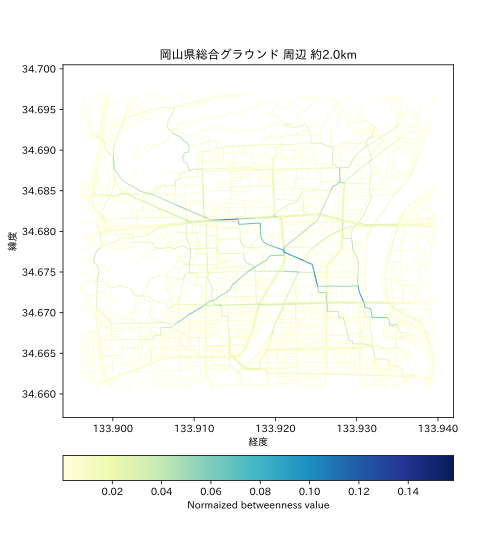
\includegraphics[width=.6\textwidth]{road-oka-with-betweenness.png}
  \caption{実験で用いる道路ネットワーク}
  \label{fig:road-okayama}
\end{figure}

図\ref{fig:road-okayama}のネットワークのひとつの辺を操作することによって各頂点の
媒介中心性を変化させる.ネットワークから削除する辺は全ての辺$14820$本が対象で,挿入する辺は
経度と緯度の平面上において,既存のどの辺とも交わらないような辺の中から$9067$本を選択した.

図\ref{fig:exp-road-betweenness-max}はそれぞれの辺操作後の媒介中心性の
最大値の分布を表す.
最大$0.1607$の正規化された媒介中心性を
辺の挿入によって最大$0.1727$に増加,辺の削除によって最大$0.1027$に減少させることに成功した.
% 辺\{4153334442,5358091035\}を挿入,辺\{5358095473,5389817383\}を削除することによって達成される

\begin{figure}[tb]
  \centering
  \includegraphics{exp-road-betweenness-max.png}
  \caption{辺操作時の媒介中心性の最大値の変化量.直線は操作前の媒介中心性の最大値($0.1607$)を表す.}
  \label{fig:exp-road-betweenness-max}
\end{figure}

図\ref{fig:road-oka-minimal-betweenness}と\ref{fig:road-oka-maximal-betweenness}は
それぞれ,正規化された媒介中心性を最大,最小にするような辺操作後の,
各頂点の正規化された媒介中心性の値の変化量を示す.

\begin{figure}[tb]
   \begin{minipage}{0.48\textwidth}
     \centering
     \includegraphics[width=.95\linewidth]{road-oka-minimal-betweenness.png}
     \caption{媒介中心性の最大値を最小にする削除辺と媒介中心性の値の変化量}
     \label{fig:road-oka-minimal-betweenness}
   \end{minipage}\hfill
   \begin{minipage}{0.48\textwidth}
     \centering
     \includegraphics[width=.95\linewidth]{road-oka-maximal-betweenness.png}
     \caption{媒介中心性の最大値を最大にする挿入辺と媒介中心性の値の変化量}
     \label{fig:road-oka-maximal-betweenness}
   \end{minipage}
\end{figure}

% \section{媒介中心性のリアルタイム計算}
% 
% 第\ref{chap:introduction}章は,社会ネットワークの分析に媒介中心性が用いられることを説明した.
% しかし,現実の社会ネットワークでは,友人関係の出現や消滅が時間とともに繰り返される.
% そのようなネットワークに対して,リアルタイムに媒介中心性を計算することは,
% 社会ネットワークの解析の観点から有用であると考えられる.
% この実験では,友人関係の出現と消滅が頻繁に発生する状況において,
% 提案手法を用いて媒介中心性をリアルタイムに計算する.
% 
% この実験では,SFHH conference data set\cite{Genois2018}というデータセットを用いた.
% このデータセットは,2009年にフランスで開催されたSFHHと呼ばれる会議の参加者に
% 赤外線タグを持たせることによって,参加者同士の交流の発生を記録したものである.
% データは20秒ごとに取得され,それぞれの時刻でどの参加者同士が近接しているかが保存されている.
% ネットワークの頂点数は$405$,辺の総数は$3509$である.
% 
% 図\ref{fig:exp-sfhh}はデータセットをもとに辺の挿入と削除を繰り返したときの,
% 提案手法とBrandes法の実行時間を表す.
% それとともに,20秒間のうちに発生した挿入辺数および削除辺数を示す.
% 図\ref{fig:exp-sfhh}より,小規模な場合ではあるが,提案手法は媒介中心性をリアルタイムに
% 計算できることが確認できる.
% しかし,更新の量が多い場合,Brandes法の方が高速に計算していることが分かる.
% 今後は,多くの辺の操作に対応するアルゴリズムの開発が求められる.
% 
% \begin{figure}[tb]
%   \centering
%   \includegraphics{exp-sfhh.png}
%   \caption{各時刻に対する各アルゴリズムの計算時間と挿入または削除された辺数.}
%   \label{fig:exp-sfhh}
% \end{figure}

\chapter{結論}

\chapter*{謝辞}
ありがとうございました.

\appendix

\printbibliography[title=参考文献]

\end{document}
